% \VignetteIndexEntry{Quick Tutorial}
% \VignetteDepends{sendplot}
% \VignetteKeyword{sendplot}
% \VignetteKeyword{tutorial}
% \VignetteKeyword{wrappers}

\documentclass[]{article}

\title{A tutorial for the sendplot R package}
\author{Lori A. Shepherd, John A. Kirchgraber Jr., and Daniel P. Gaile}

\usepackage{/projects/aCGH/Active/CodeDevelopment/R/lib/R/share/texmf/Sweave}
\begin{document}

\maketitle

\begin{center}
Statistical Genetics and Genomics Research Group\\
Department of Biostatistics, University at Buffalo\\
New York State Center of Excellence in Bioinformatics and Life Sciences
\end{center}

\begin{center}

{\tt las65@buffalo.edu}
\end{center}


\tableofcontents

\section{Introduction}


\indent The functions in the sendplot library allow R users to generate interactive plots with tool-tip content. A pair of files are created : a Portable Network Graphics (PNG) file which is a bitmap image and an HTML file which contains embedded Javascript code for dynamically generating tool-tips. When opened with a supported browser, the HTML file displays the PNG image and the user is able to mouse over and view tool-tip windows for user specified image locations. The information that appears in the tool-tip windows is user specified and highly customizable. The tool-tip functionality is provided by code from the  wz\_tooltip.js Javascript library (Zorn 2007) which is embedded in the HTML output.



\indent The 'sendplot' function constitutes the primary function of the sendplot library. It allows for the generation of interactive xy (i.e., scatter-plot) and image (i.e., heatmap) plots, which can contain any number of decorative (i.e., non-interactive) plots. The library also contains three convenient wrapper functions: sendxy, sendimage, and heatmap.send. The wrapper functions have less functionality than the sendplot function but can be easier to use. Brief descriptions of the four functions are as follows:

\begin{itemize}
\item sendxy : this function produces an interactive xy plot without any decorative plots (i.e., just a single scatter-plot).
\item sendimage :  this function produces an interactive image plot without any decorative plots (i.e., just a single image plot).
\item heatmap.send : this function is a wrapper for the R stats package heatmap. This will
create an interactive heatmap image. NOTE: The majority of the code for
this function is verbatim from the R package stats heatmap
function. This function was designed to work as a wrapper to utilize
the same functionality and plotting as the heatmap function with
sendplot's interactive functionality.
\item sendplot: this function produces an interactive xy or image plot which is an element of layout which can contain other decorative plots. 
\end{itemize}


\indent The creation of interactive plots with tool-tip content requires the development of the following components:
\begin{description}
\item 1. The static plot image. The library supports the following: a simple xy-plot (sendxy), a simple image plot (sendimage), a heatmap with decorative dendrograms (heatmap.send), or a flexible layout of plots which contains one interactive xy-plot or image plot (sendplot). The functions in the sendplot library allow for the full complement of graphical bells and whistles which are available in R (e.g., custom axes, inclusion of legends, math symbols, etc.). 
\item 2. The plotted point to pixel mapping. The sendplot functions output an HTML file and a PNG image. The HTML file contains an image map which identifies the interactive regions of the PNG image (i.e., the regions for which a tool-tip will appear). The image map requires a mapping of the plotted point coordinates as specified in the R plotting calls that generated them to the corresponding pixel location on the final PNG image. The sendplot functions build this map by identifying the upper-left and lower-right locations in the original plotting coordinate system and in the final pixel coordinate system. The functions provide a convenient mechanism to accomplish this.
\item 3. The tool-tip content lists. The sendplot functions allow users to specify  x-specific, y-specific, and point specific (e.g., xy-specific) information to be displayed in the tool-tip. 
\end{description}
The sendplot functions are typically run in two iterations when creating interactive plots for the first time. In the first iteration, the PNG file is created and then opened in a program such as mspaint or kolourpaint so that the upper-left and lower-right pixel coordinates are identified. In the second iteration, the function is called again using the pixel coordinates identified in the first iteration and the PNG and HTML output files are created. Figure 1 provides a flowchart for this two-iteration procedure. {\bf{Note:}} the first iteration need not be repeated for calls that use the sample plot type and output image size as the upper-left and lower-right pixel will not change. \newline
\indent For linux/unix users, there is an option for automatic detection of the upper-left and lower-right pixil coordinates. This utilizes ImageMagick's convert program installed on most linux machines, and the R library rtiff's readTiff function. This eliminates the need for a second interaction. For windows/mac users, this automatic detection of coordinates is viable if the user has the ability to convert a PNG image to a TIFF image; two iterations are still needed. The first iteration will create the PNG images. The user manually converts the PNG images to the TIF images using appropriate file names. The function is run again and the auto detect will function correctly.  


\begin{center}
\begin{figure}
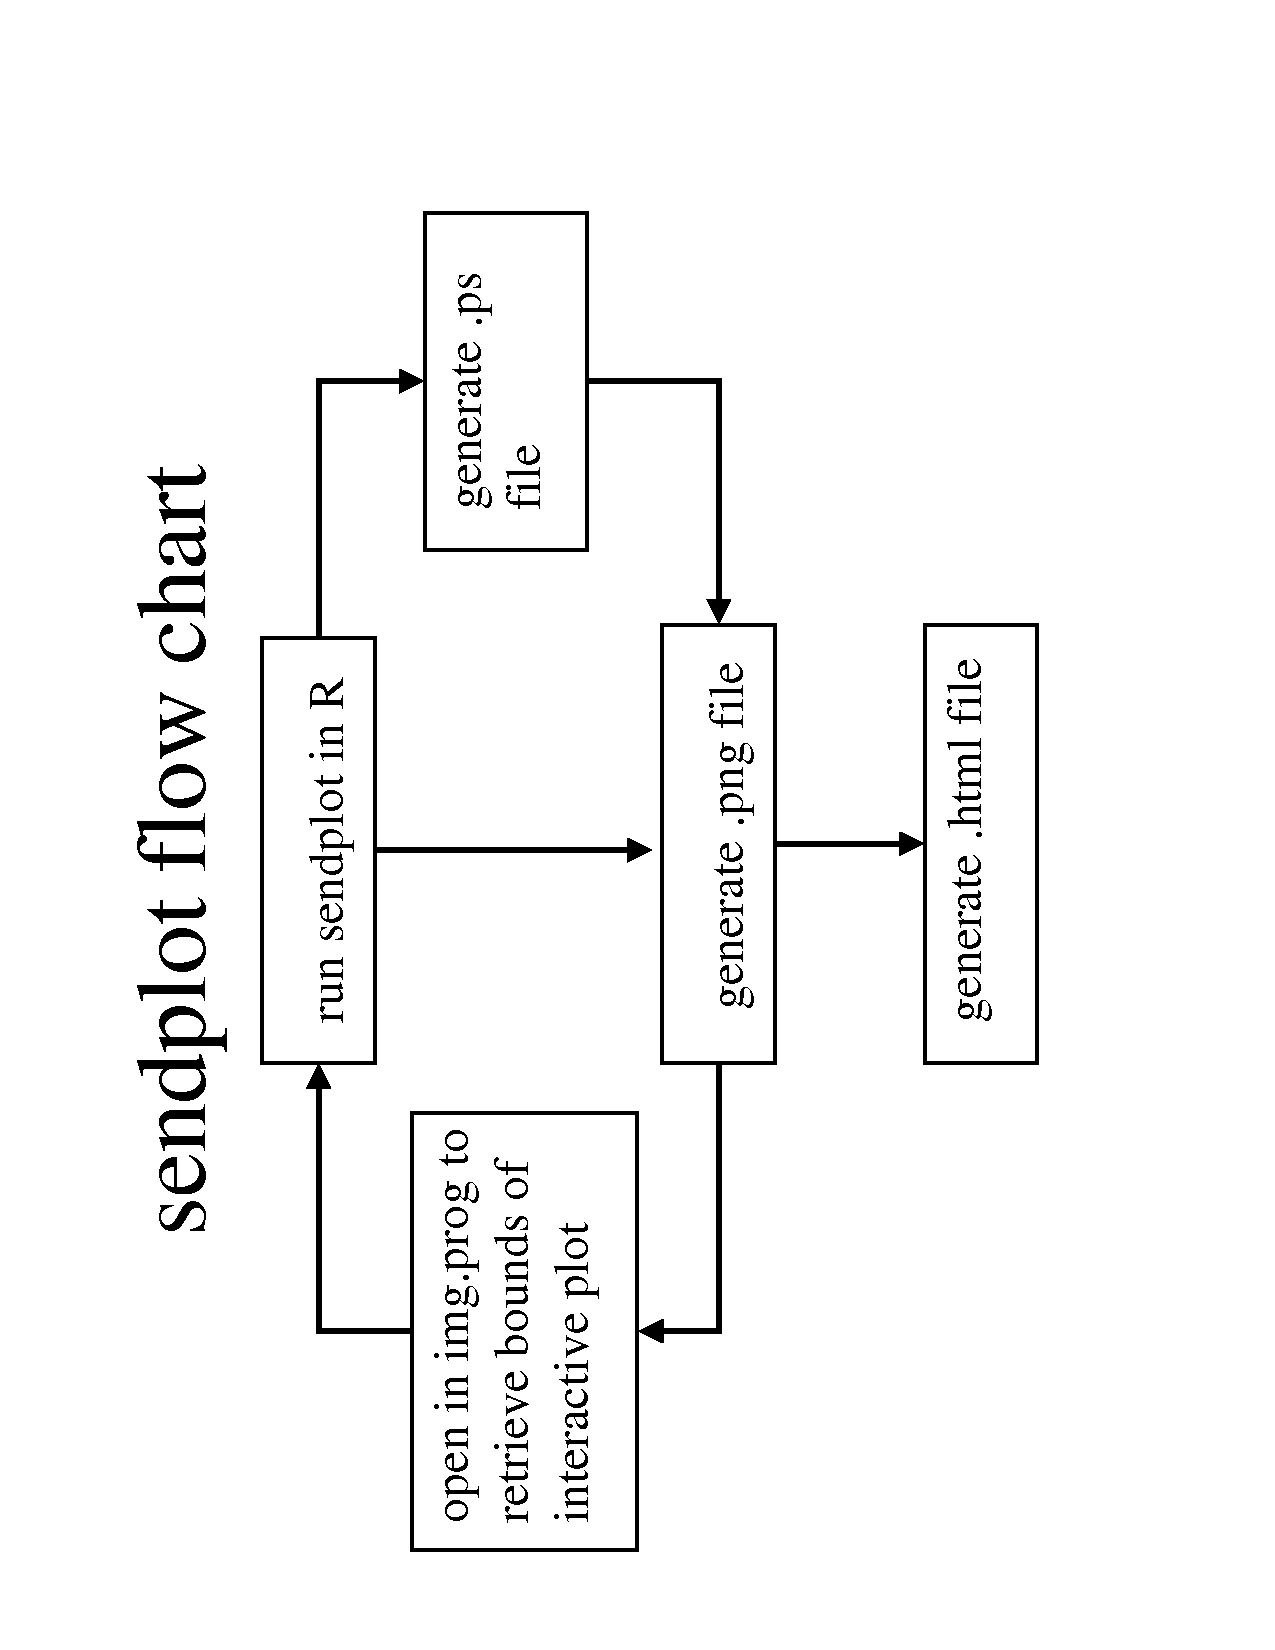
\includegraphics[angle=270]{sendplotFlowChart}
\caption{The sendplot functions are typically run in two iterations when creating interactive plots for the first time. The first iteration involves the identification of the upper-left and lower-right pixel coordinates. The final output is generated in the second iteration.An option has bee implimented to eliminate this two step procedure for linux/unix machines.}
\end{figure}
\end{center}


\indent The remainder of this document will provide detailed tutorials for the use of the functions: sendxy, sendimage, heatmap.send, and sendplot. All sections assume library has been loaded:

\begin{Schunk}
\begin{Sinput}
> library(sendplot)
\end{Sinput}
\end{Schunk}

\vskip5mm
\indent{\bf{Important Note:}} The sendplot output has been tested on Firefox and Internet Explorer browsers.  Internet Explorer users may need to modify their preferences to allow blocked content, as Internet Explorer may initially block the scripts from running. A warning message normally appears towards the top of the browser; if the user click on this warning it will give an option to allow blocked content.


%\newpage

\section{sendxy: scatter-plot wrapper}

The sendxy function creates a single interactive scatter-plot. The following is an example function call:
\begin{verbatim}
     sendxy(plot.call,
            x, y, 
            xy.lbls = NA, x.lbls = NA,y.lbls=NA,
            xlim = NA, ylim = NA,
            mai=NA, mai.prc=FALSE,plt.extras=NA,
            bound.pt=FALSE, source.plot=NA,
            paint=FALSE,img.prog = NA,
            resize="800x1100",
            ps.paper="letter",ps.width=8,ps.height=11,
            fname.root="test",dir="./",header="v2",
            up.left=c(205,131),low.right=c(633,883),
            spot.radius=5, automap=FALSE, automap.method="mode")
 \end{verbatim}


\subsection{specifying the plot call}
The plot.call argument is a character string containing the call for the desired scatter-plot. For example, consider the two datasets: the first containing identical x and y values ranging from 1 to 7 and the second containing x values decreasing from 7 to 1 with a constant y value of 4.

\begin{verbatim}
x1 = 1:7
y1 = 1:7  
x2 = 7:1
y2 = rep(4,7)
\end{verbatim}

The following example plot.call argument will plot the first dataset as a green plus and the second as a purple X. 

\begin{verbatim}
plot.calls = "plot(x1,y1,col='green', pch=3, cex=1.5,xlab='',ylab='');
              points(x2,y2,pch=4, cex=1.5, col='purple');
              title(xlab='x values', ylab='y values')"
\end{verbatim}



Notice how the call is a character string that will be evaluated as multiple function calls separated by a semicolon. Arguments of type character within these calls are specified with a single quotation rather than the double quotations used originally, or vice versa (see col arguments). Any variables used in arguments (x1,x2,y1,y2 in our example) should be in local memory before running the sendxy function call. \\ \indent NOTE: No xlim or ylim value should be specified in any of the plot.call plotting calls. For mapping purposes, xlim and ylim must be given as separate arguments to the function. If xlim and ylim are not set in the arguments, or entered as NA, the range of the x and y values will be used. \newline

\indent mai and mai.prc control the plot margins. If mai is NA (default), the application uses default plot margins. For more information on mai, mai.prc, plt.extras, and header please refer to R help files or to the last section of this vignette (i.e., the sendplot section). \newline

\subsection{specifying the interactive points and tool-tip content}

\indent The x and y arguments are the x and y coordinates of desired interactive points. If, for example, we only wanted the points of the first dataset to be interactive: x = x1 and y = y1.  If, however, we want all the points of both datasets to be active, the x and y should be a combination of all datasets' x and y values.  
\begin{verbatim}
 x = c(x1,x2)
 y = c(y1,y2)
\end{verbatim}

\indent The arguments x.lbls, y.lbls, and xy.lbls control what is displayed in the interactive window when the user hovers the mouse over plot points. The arguments x.lbls and y.lbls refer to data that is specific to the x and y values respectively. The argument xy.lbls governs data specific to both x and y location. In the case of a scatter-plot, x.lbls, y.lbls, and xy.lbls refer to the same position; it is only necessary to use either x.lbls or y.lbls. x.lbls and y.lbls are data.frames with the number of rows equal to the number of interactive data points. The first row of the data frame should contain column headers; these names will be used as display names in the interactive window that appears. \newline
\indent For our example, we have 14 data points. The following creates a data.frame of information for the 14 data points; each point has a letter and a number associated with it. 
\begin{verbatim}
  x.lbls = list()
  x.lbls$letter = rep(c("a","b","c","d","e","f","g"),2)
  x.lbls$number = 1:14
  x.lbls = as.data.frame(x.lbls)
\end{verbatim}
\begin{Schunk}
\begin{Soutput}
   letter number
1       a      1
2       b      2
3       c      3
4       d      4
5       e      5
6       f      6
7       g      7
8       a      8
9       b      9
10      c     10
11      d     11
12      e     12
13      f     13
14      g     14
\end{Soutput}
\end{Schunk}
\indent {\bf{Note:}} the function assumes the data.frame rows are in the same order as they appear in the x argument (or y argument if y.lbls).  \newline


\subsection{creating the PNG image file}

The following arguments play a role in the generation of the final PNG image file:
\begin{description}
  \item{source.plot:~}{Indicates whether application should make a
    postscript file and then convert to png file, or if the png file
    should be made directly. This value is either ps, png, or NA. If NA
    the operating system is checked and the appropriate file format is
    output. Unix has a convert function that can convert a ps file to
    png file; we by default use this setup because we feel the
    postscript file maintains better quality. So on unix/linux systems
    if source.plot is NA, source.plot will be set to ps. Windows does
    not have this option, for this reason source.plot will be set to png
    if left NA}

  \item{dir:~}{directory path to where files should be created}
  \item{fname.root:~}{Base name to use for postscript, .png, and html
    file names.}

  \item{resize:~}{character indicating resize value. If source.plot is "ps", resize is passed as part of a system convert command converting the postscript to the .png. The original image is resized to this dimension expanding condensed images or vice versa. If source.plot is "png", the argument is parsed and the dimensions are passed into the R grDevices package function png as the width and height arguments.}
  \item{ps.paper:~}{postscript paper argument}
  \item{ps.width:~}{postscript width argument (only used if ps.paper=''special'')}
  \item{ps.height:~}{postscript height argument (only used if ps.paper=''special'')}


\end{description}
The source.plot argument controls what file formats are created. The interactive html file requires a .png file. There are two possible scenarios for making a .png file: the .png file may be made directly, or a postscript file may be made first and then converted into a .png file. We recommend making the postscript file and converting to the .png file because it maintains better clarity and quality.


\indent If the source.plot argument is set to "png" then a PNG file is generated directly. If the source.plot argument is set to "ps" then a postscript file is generated and then converted (using the 'convert' command in linux or a user specified application in windows) to the PNG format. The ps.paper, ps.width, and ps.height arguments specify the dimensions of the postscript output. If the ps.paper argument is set to a recognized format such as ``letter'' or ``a4'', then the ps.width and ps.height arguments are ignored. If the ps.paper argument is set to ``special'' then the postscript dimensions are governed by ps.height and ps.width. 



\subsection{creating the image map}

As mentioned previously, the sendplot functions output an HTML file and a PNG image. The HTML file contains an image map which identifies the interactive regions of the PNG image (i.e., the regions for which a tool-tip will appear). The image map requires a mapping of the plotted point coordinates as specified in the R plotting calls that generated them to the corresponding pixel location on the final PNG image. The sendplot functions build this map by identifying the upper-left and lower-right locations in the original plotting coordinate system and in the final pixel coordinate system. The function arguments for these coordinates are given as:
\begin{description}
  \item{up.left:~}{The x and y value in pixels of the upper left hand
    corner of the plot call}
  \item{low.right:~}{The x and y value in pixels of the lower right hand
    corner of the plot call.}
\end{description}

\indent The sendplot functions provide convenient options for identifing the upper-left and lower-right pixil coordinates. There is an automatic detection of bounding points, in most cases eliminating the two step procedure. There are also options for manual detection of bound points. These options will be discussed further in the following sections.  

\subsubsection{automatic dectection of bounding points}

\indent As mentioned previously, there is an option for automatic detection of the upper-left and lower-right pixil coordinates. This option eliminates the two iteration procedure for linux and unix users. The functions utilizes ImageMagick's convert program installed on most linux machines, and the R library rtiff's readTiff function. The function arguments implementing this option are:
\begin{description}
 \item{automap:~}{logical indicating if application should
    attempt to automatically detect upper-left and lower-right 
    coordinates.}

  \item{automap.method:~ }{if automap is TRUE, the method that will be
    used to find bound points. The current options are median and mode}

 \end{description}

\indent For windows and mac users, this automatic detection of coordinates is viable if the user has the ability to convert a PNG image to a TIFF image. The current implemenation still requires two iterations. The first iteration will create the PNG images. The user then must manually convert the PNG images to the TIF images using appropriate file names. The function is run again and the auto detect will function correctly.  

\indent Continuing the current example, the following code is executed:
\begin{verbatim}
sendxy(plot.call=plot.calls, 
              x=x, y=y,
              x.lbls=x.lbls, 
              source.plot=NA, 
              automap=TRUE, automap.method="mode",
              fname.root="testXY",resize="800x1100",
              up.left=c(205,131),low.right=c(633,883))
\end{verbatim}


\subsubsection{manual detection of bounding points}

\indent As mentioned previously, the sendplot functions are typically run in two iterations when creating interactive plots for the first time. In the first iteration, the PNG file is created and then opened in a program such as mspaint or kolourpaint so that the upper-left and lower-right pixel coordinates are identified. In the second iteration, the function is called again using the pixel coordinates identified in the first iteration and the PNG and HTML output files are created.  Refer back to Figure 1 for a flowchart for this two-iteration procedure. 


\indent The sendplot functions  include arguments which allow for the convenient identification of the up.left and low.right values. These arguments are:

\begin{description}
 \item{paint:~}{logical indicating if application should
    automatically open the .png file for the user to view .png file and/or
    to retrieve needed bounding values of the plot call.}

  \item{img.prog:~ }{if paint is TRUE, the command line call that will open
    a program to view .png file to retrieve pixel locations of interactive
    plot bounds. If this is left NA, the operating system is checked and
    a default program is used. For unix the default application is
    kolourpaint and for windows it is Microsoft paint (mspaint).}

  \item{bound.pt:~}{logical indicating if red points should be plotted to
    aid in finding the upper left and lower right coordinates. If
    bound.pt is FALSE, indicates that up.left and low.right arguments
    are correct and will make the html file. Note that if bound.pt is TRUE then the function will not
    attempt the task of writing the .html file as that step can be time consuming.}

 \end{description}
One way to identify the up.left and low.right values in the first iteration of sendplot construction is to execute the function with: bound.pt=TRUE, paint=TRUE, and img.prog=NA. With this combination of arguments, the function will create the PNG output, add red points to the upper-left and lower-right corners, and then open the PNG in the default viewer so that the user can readily identify the up.left and low.right pixel coordinates. 

\indent Continuing the current example, the following code is executed:
\begin{verbatim}
sendxy(plot.call=plot.calls, 
              x=x, y=y,
              x.lbls=x.lbls, 
              bound.pt=TRUE, 
              source.plot=NA, paint=TRUE,
              img.prog=NA,
              fname.root="testXY",resize="800x1100",
              up.left=c(205,131),low.right=c(633,883))
\end{verbatim}
We have entered dummy values for the up.left and low.right coordinates. Figure 2 contains a screenshot of the example PNG file opened in kolourpaint. According to the information in kolourpaint, the up.left location should be 124,130. Notice the mouse is over the upper left red point for the up.left bounding box. The pixel location is shown on the bottom of the window in the second box from the left. It shows a location of 124, 130. If we had checked the low.right coordinate it would read 713,885. To complete the process of generating the sendxy output, the sendxy function used to created this figure should be rerun with bound.pt=FALSE, paint=FALSE,up.left=c(124,130) and low.right=c(713,885). \newline



\begin{center}
\begin{figure}
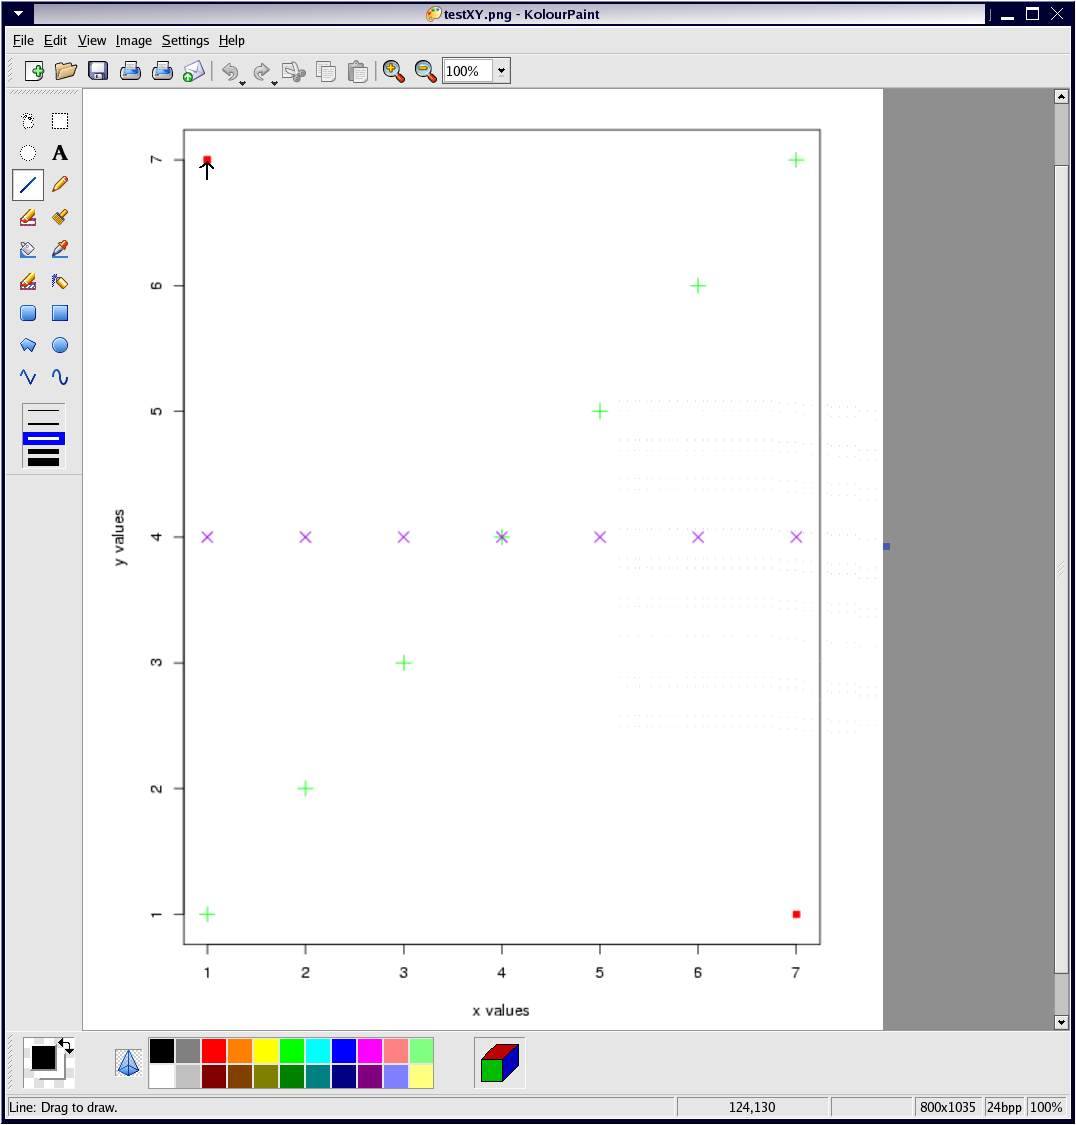
\includegraphics{scatterPaint}
\caption{scatter-plot opened in kolourpaint, showing additional red points to aid in locating boundaries. Notice where pixel location can be found}
\end{figure}
\end{center}

NOTE: As mentioned earlier, the sendxy function does not always need to be run iteratively. If the user is using the same machine (therefore consistent point size and operating system), the plot's xlim, ylim, and margins are the same, and the resize value is the same, the bounding points will also be the same. Helpful hint:  In may cases if the user is generating similar plots, the xlim and ylim can be set constant so that all graphs are on the same scale; mai=NA using the default margins will also be consistent. This process of retrieving bound.pt needs to be performed once for a certain group of settings.\newline
\\


\subsection{specifying the spot radius}

\indent The spot.radius argument controls how large an area will be active when the mouse is scrolled over. If the user selects a larger region, some spot locations may overlap and be lost. The interactive application is very sensitive if the user selects a low region. The users' discretion is best used here given that the plot scale and number of data points will also play a role in determining a good spot.radius.  \\

\subsection{creating the sendxy example output}

\indent If automap is used to detect bounding points the function automatically continues making the HTML file and sendxy final example output. 

\indent If bounding points are detected manually, after the correct bounding points are known, the sendxy function call should be run again, changing only the up.left, up.right, paint, and bound.pt arguments. up.left and low.right should be updated accordingly. paint and bound.pt should be tripped to FALSE. (NOTE: these are the correct up.left and low.right boundaries when the .png is created from the postscript in linux/unix environment. If the .png file was generated directly the up.left and low.right values of this example may be slightly different).  The following will make the correct interactive plot:
\begin{verbatim}
# manual detection of points  
sendxy(plot.call = plot.calls, 
       x=x, y=y,
       x.lbls=x.lbls,  
       bound.pt=FALSE, 
       source.plot=NA, paint=FALSE,
       img.prog=NA,fname.root="testXY",resize="800x1100", 
       up.left=c(124,130),low.right=c(713,885), spot.radius=5)

# or 
# automatic detection of points
sendxy(plot.call = plot.calls, 
       x=x, y=y,
       x.lbls=x.lbls,  
       source.plot=NA, 
       automap=TRUE, automap.method="mode"
       fname.root="testXY",resize="800x1100", 
       up.left=c(124,130),low.right=c(713,885), spot.radius=5)
\end{verbatim}


The resulting HTML file may be opened in any web browser that is capable of running Javascript. Figure 3 shows a snapshot of the final graph opened in Mozilla Firefox. Notice how the appropriate information for the region located under the white arrow is displayed in the information box.
\begin{center}
\begin{figure}
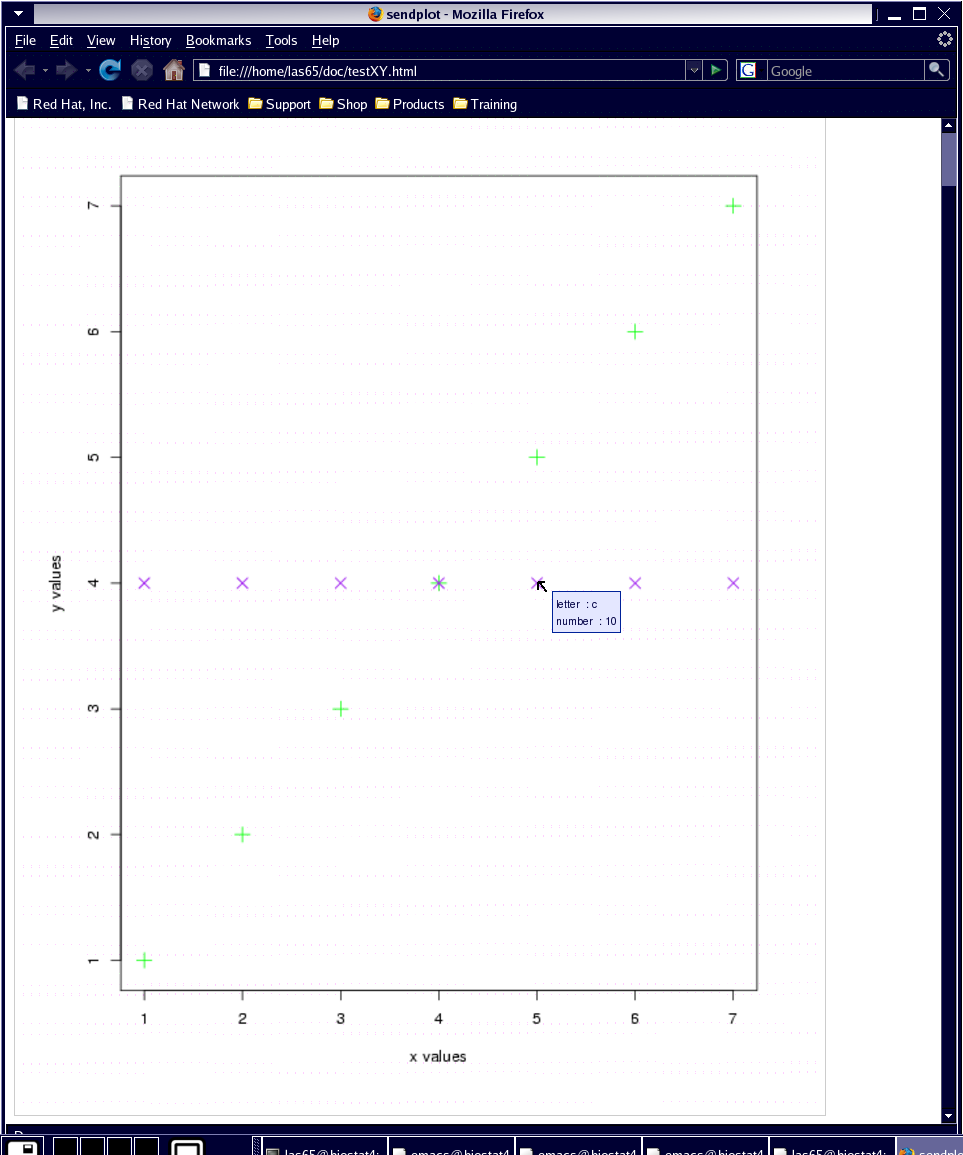
\includegraphics{sendPlotScatter}
\caption{A snapshot of our example html file opened in Mozilla Firefox. The information is displayed for the region under the black arrow.}
\end{figure}
\end{center}



\subsection{summary of code used to generate the sendxy example}

 The following is a summary of all code run to make the above example:

\begin{verbatim}
  library("sendplot")
	 
  x1 = 1:7
  y1 = 1:7    
  x2 = 7:1
  y2 = rep(4,7)
  x = c(x1,x2)
  y = c(y1,y2)

  xy.lbls = list()
  xy.lbls$test = rep(c("a","b","c","d","e","f","g"),2)
  xy.lbls$num = 1:14
  xy.lbls = as.data.frame(xy.lbls)
	    
  plot.calls = "plot(x1,y1,col='green', pch=3, cex=1.5,xlab='',ylab='');
                points(x2,y2,pch=4, cex=1.5, col='purple');
                title(xlab='x values', ylab='y values')"
   

#automatic detection of bound points

sendxy(plot.call = plot.calls, 
       x=x, y=y,
       x.lbls=x.lbls,  
       source.plot=NA, 
       automap=TRUE, automap.method="mode"
       fname.root="testXY",resize="800x1100", 
       up.left=c(124,130),low.right=c(713,885), spot.radius=5)

# or 

# manual detection bound points

  sendxy(plot.call = plot.calls, 
         x=x, y=y,
         x.lbls=xy.lbls, 
         plt.extras=NA,
         bound.pt=TRUE, 
         source.plot=NA, paint=TRUE,
         img.prog=NA,fname.root="testXY",resize="800x1100",
         up.left=c(205,131),low.right=c(633,883))

# correct bounding found (124,130), (713,885)

  sendxy(plot.call = plot.calls, 
         x=x, y=y,
         x.lbls=xy.lbls, 
         plt.extras=NA,
         bound.pt=FALSE, 
         source.plot=NA, paint=FALSE,
         img.prog=NA,fname.root="testXY",resize="800x1100",
         up.left=c(124,130),low.right=c(713,885), spot.radius=5)
 
\end{verbatim}


And there you have it, an interactive scatter-plot! 

\newpage



\section{sendimage: image wrapper}

The sendimage function creates a single interactive image. The following is an example function call: 

\begin{verbatim}
     sendimage(plot.call,
               x, y, z,
               z.value="value",
               x.lbls = NA,y.lbls=NA,xy.lbls=NA,
               mai=NA, mai.prc=FALSE,plt.extras=NA,
               bound.pt=FALSE, source.plot=NA,
               paint=FALSE, img.prog=NA,
               resize="800x1100",
               ps.paper="letter",ps.width=8,ps.height=11,
               fname.root="test",dir="./",header="v2",
               up.left=c(188,103),low.right=c(648,912),
               spot.radius=5, automap=FALSE, automap.method="mode")
\end{verbatim}

For the most part the arguments for sendimage are consistent with those for sendxy. 

\subsection{specifying the plot call}
As with the sendxy function, the plot.call argument is a character string containing the call for the desired image plot. Consider the following example data corresponding to a 4 x 5 image:
\begin{verbatim}
x = 1:4
y = 1:5
z = t(matrix(round(rnorm(20),digits=3), ncol=4))
\end{verbatim}



The following constructs a plot.call argument for the desired image. 

\begin{verbatim}
plot.calls = "image(x=x, y=y, z=z);title(main='sendimage example')"
\end{verbatim}


Notice how the call is a character string that will be evaluated as multiple function calls separated by a semicolon.  Arguments of type character within these calls are specified with a single quotation rather than the double quotations used originally, or vice versa (see main argument). Any variables used in arguments (x,y,z in our example) should be in local memory before running the sendimage function call. \newline


\indent mai and mai.prc control the plot margins. If mai is NA (default), the application uses default plot margins. For more information on mai, mai.prc, plt.extras, and header please refer to R help files or to the last section of this vignette (i.e., the sendplot section). \newline


\subsection{specifying the interactive points and tool-tip content}

\indent The x, y, and z arguments are the x, y, and z used in the image call. x and y are the locations of the grid lines at which the values of z correspond. z is a matrix of values (length of x  by length of y). The function argument z.value describes what z holds (examples pvalues, logRatios, percentAccepted); this identifier is used in the interactive display. These three arguments have already been defined in the previous section. \\

\indent {\bf{Note:}} z.value should not contain any spaces or punctuation characters; numbers and letters only.

\indent As with the sendxy function, the arguments x.lbls, y.lbls, and xy.lbls control what is displayed in the interactive window when the user hovers the mouse over plot points. The arguments x.lbls and y.lbls refer to data that is specific to the x and y values respectively. x.lbls and y.lbls are data.frames of the dimension n by m, where n is equal to the length of x or y respectively. Each row is specific to a certain x or y value and each column is a unique variable or characteristic of x or y respectively.  The first row of the data frames should contain column headers; these names will be used as display names in the interactive window that appears. The xy.lbls argument is a little different because it governs data specific to both x and y locations. The function argument xy.lbls is a list of matrices; each matrix is of the dimension n by m, where n is equal to the length of y and m is equal to the length of x.\\ 

\indent Consider an example dataset which contains clinical and experimental data corresponding to 4 tissue samples. The experimental data is derived from BAC array comparative genomic hybridization experiments from which the results for five particular BAC assays are considered here. Hence, the experimental data for this example dataset is a 4x5 data matrix of observed (real valued) log2 tumor/control ratios. Each of the BAC assays has attributes such as chromosome location, genomic location. Each of the samples has attributes such as sex, age, and tumor stage. The x.lbls data.frame is 4 x 3: 4 patients, 3 characteristics based on patients (sex, age, stage). The y.lbls data.frame is a 5 x 2: 5 events, 2 characteristics (chromosome, genomic location).  The xy.lbls is a list of length 2: 2 additional pieces of data collected: intensity and quality control measure. Each of these two objects is a 5 x 4 matrix: 5 BACs, 4 patients. Our log2 ratios data is already set as z. The set up of the x.lbls, y.lbls and xy.lbls objects would be something like the following:

\begin{verbatim}
x.lbls = list()
x.lbls$sex = c("F", "M", "F", "F")
x.lbls$age = c(27, 73, 46, 50)
x.lbls$stage = c(1,1,3,2)
x.lbls = as.data.frame(x.lbls)

y.lbls = list()
y.lbls$chromosome = c("chr1", "chr2", "chrX", "chr7", "chrY")
y.lbls$location = c(92526, 486844000,2984248632,1387071184,3048286585)

xy.lbls = list()
intensity = matrix(c(-.3,1.0,.3,-.07,-.4,1.2,.4,.3,1.0,-.5,-.06,1.1,
                     .04,.5,.03,-.09,-.04,.06,.01,.03),nrow=5)
xy.lbls$intensity = intensity
QC = matrix(c(T,T,T,T,T,F,T,T,T,F,T,T,T,T,T,F,T,F,T,T), nrow=5)
xy.lbls$QC = QC

\end{verbatim}


\indent {\bf{Note:}} the function assumes the data.frame rows are in the same order as they appear in the x argument (or y argument if y.lbls).  \newline
\indent {\bf{Note:}} z values automatically display in the interactive window. If x.lbls, y.lbls, and xy.lbls are NA, the interactive window will only display z values. 


\subsection{creating the PNG image file}

\indent sendimage follows the same process as sendxy for creating the PNG image file. Please refer to section 2.3 for details.

\subsection{creating the image map}

As mentioned previously, the sendplot functions output an HTML file and a PNG image. The HTML file contains an image map which identifies the interactive regions of the PNG image (i.e., the regions for which a tool-tip will appear). The image map requires a mapping of the plotted point coordinates as specified in the R plotting calls that generated them to the corresponding pixel location on the final PNG image. The sendplot functions build this map by identifying the upper-left and lower-right locations in the original plotting coordinate system and in the final pixel coordinate system. The function arguments for these coordinates are given as:
\begin{description}
  \item{up.left:~}{The x and y value in pixels of the upper left hand
    corner of the plot call}
  \item{low.right:~}{The x and y value in pixels of the lower right hand
    corner of the plot call.}
\end{description}

\indent The sendplot functions provide convenient options for identifing the upper-left and lower-right pixil coordinates. There is an automatic detection of bounding points, in most cases eliminating the two step procedure. There are also options for manual detection of bound points. These options will be discussed further in the following sections.  

\subsubsection{automatic dectection of bounding points}

\indent As mentioned previously, there is an option for automatic detection of the upper-left and lower-right pixil coordinates. This option eliminates the two iteration procedure for linux and unix users. The functions utilizes ImageMagick's convert program installed on most linux machines, and the R library rtiff's readTiff function. The function arguments implementing this option are:
\begin{description}
 \item{automap:~}{logical indicating if application should
    attempt to automatically detect upper-left and lower-right 
    coordinates.}

  \item{automap.method:~ }{if automap is TRUE, the method that will be
    used to find bound points. The current options are median and mode}

 \end{description}

\indent For windows and mac users, this automatic detection of coordinates is viable if the user has the ability to convert a PNG image to a TIFF image. The current implemenation still requires two iterations. The first iteration will create the PNG images. The user then must manually convert the PNG images to the TIF images using appropriate file names. The function is run again and the auto detect will function correctly.  

\indent Continuing the current example, the following code is executed:
\begin{verbatim}
 sendimage(plot.call = plot.calls, x=x, y=y, z=z,z.value='value',
            x.lbls = x.lbls, y.lbls=y.lbls, xy.lbls=xy.lbls,
            up.left=c(89,100),low.right=c(800,900),
            source.plot=NA,
            fname.root="testImg",resize="800x1100",
            automap=TRUE, automap.method="mode")
\end{verbatim}


\subsubsection{manual detection of bounding points}

\indent As mentioned previously, the sendplot functions are typically run in two iterations when creating interactive plots for the first time. In the first iteration, the PNG file is created and then opened in a program such as mspaint or kolourpaint so that the upper-left and lower-right pixel coordinates are identified. In the second iteration, the function is called again using the pixel coordinates identified in the first iteration and the PNG and HTML output files are created.  Refer back to Figure 1 for a flowchart for this two-iteration procedure. 


\indent The sendplot functions  include arguments which allow for the convenient identification of the up.left and low.right values. These arguments are:

\begin{description}
 \item{paint:~}{logical indicating if application should
    automatically open the .png file for the user to view .png file and/or
    to retrieve needed bounding values of the plot call.}

  \item{img.prog:~ }{if paint is TRUE, the command line call that will open
    a program to view .png file to retrieve pixel locations of interactive
    plot bounds. If this is left NA, the operating system is checked and
    a default program is used. For unix the default application is
    kolourpaint and for windows it is microsoft paint (mspaint).}

  \item{bound.pt:~}{logical indicating if blue points should be plotted to
    aid in finding the upper left and lower right coordinates. If
    bound.pt is FALSE, indicates that up.left and low.right arguments
    are correct and will make the html file. Note that if bound.pt is TRUE then the function will not
    attempt the task of writing the .html file as that step can be time consuming.}

 \end{description}
One way to identify the up.left and low.right values in the first iteration of sendplot construction is to execute the function with: bound.pt=TRUE, paint=TRUE, and img.prog=NA. With this combination of arguments, the function will create the PNG output, add blue points to the upper-left and lower-right corners, and then open the PNG in the default viewer so that the user can readily identify the up.left and low.right pixel coordinates. \\

\indent {\bf{Note:}} The upper-left and lower-right corners of an image, are the corners of the image itself, respectively.\newline

\indent Continuing the current example, the following code is executed:
\begin{verbatim}
  sendimage(plot.call = plot.calls, x=x, y=y, z=z,z.value='value',
            x.lbls = x.lbls, y.lbls=y.lbls, xy.lbls=xy.lbls,
            up.left=c(89,100),low.right=c(800,900),
            bound.pt=TRUE, source.plot=NA, paint=TRUE,
            img.prog=NA,fname.root="testImg",resize="800x1100")
\end{verbatim}

We have entered dummy values for the up.left and low.right coordinates. Figure 4 contains a screenshot of the example PNG file opened in kolourpaint. According to the information in kolourpaint, the up.left location should be 101,99. Notice the mouse is over the upper left blue point for the up.left bounding box. The pixel location is shown on the bottom of the window in the second box from the left. It shows a location of 101,99. If we had checked the low.right coordinate it would read 735,914. To complete the process of generating the sendimage output, the sendimage function used to created this figure should be rerun with bound.pt=FALSE, paint=FALSE,up.left=c(101,99) and low.right=c(735,914). \newline

\begin{center}
\begin{figure}
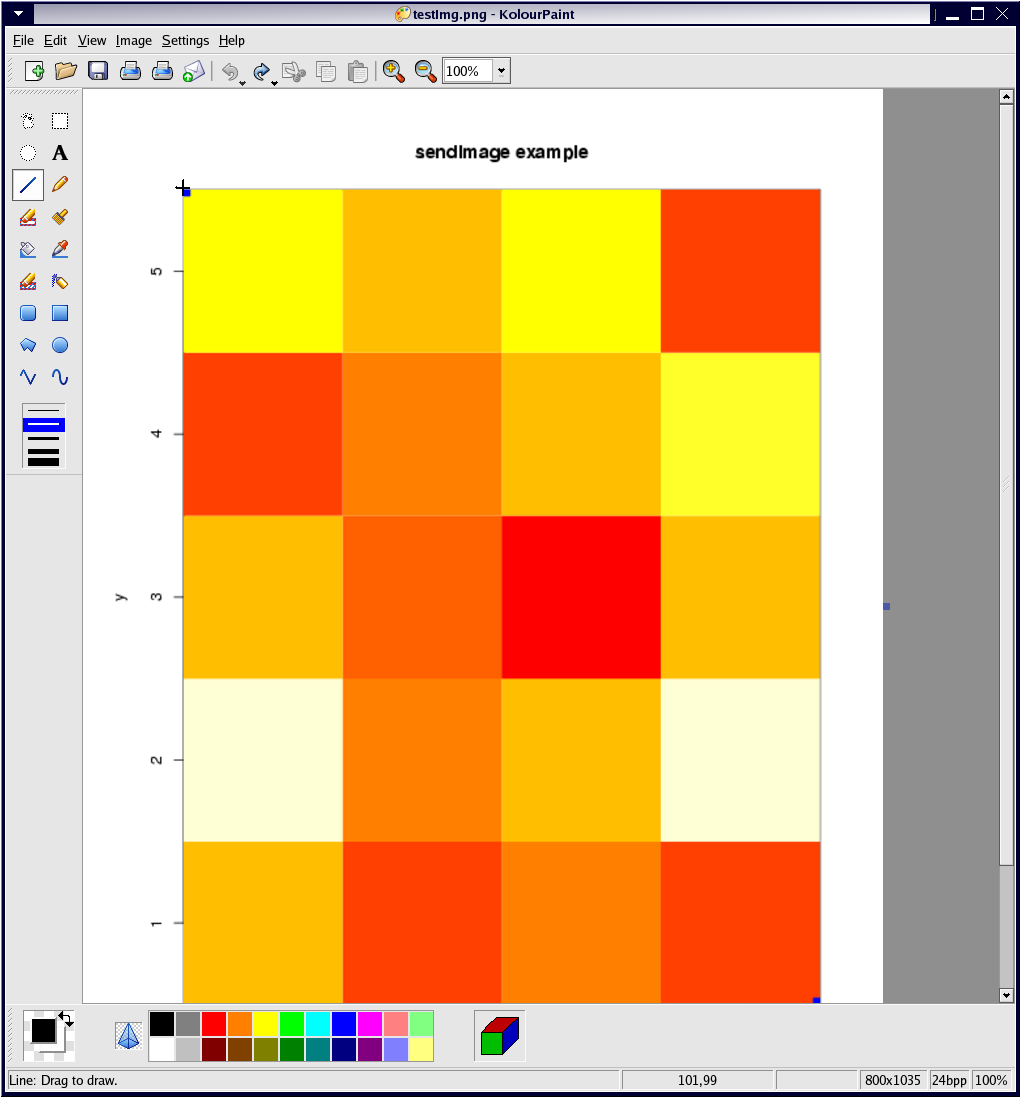
\includegraphics{imagePaint}
\caption{image opened in kolourpaint, showing additional blue points to aid in locating boundaries. Notice where pixel location can be found}
\end{figure}
\end{center}

NOTE: As mentioned earlier, the sendimage function does not always need to be run iteratively. If the user is using the same machine (therefore consistent point size and operating system), the plot's xlim, ylim, and margins are the same, and the resize value is the same, the bounding points will also be the same. Helpful hint: setting mai=NA, therefore using the default margins, will keep margins consistent. This process of retrieving bound.pt needs to be performed once for a certain group of settings.\newline
\\

\subsection{specifying the spot radius}

\indent The spot.radius argument for sendimage is the same as in sendxy. Please refer to section 2.5 for details. 

\subsection{creating the sendimage example output}

\indent If automap is used to detect bounding points the function automatically continues making the HTML file and sendxy final example output. 

\indent If bounding points are detected manually, after the correct bounding points are known, the sendimage function call should be run again, changing only the up.left, up.right, paint, and bound.pt arguments. up.left and low.right should be updated accordingly. paint and bound.pt should be tripped to FALSE. (NOTE: these are the correct up.left and low.right boundaries when the .png is created from the postscript in linux/unix environment. If the .png file was generated directly the up.left and low.right values of this example may be slightly different).  The following will make the correct interactive plot:

\begin{verbatim}
# manual detection of points
sendimage(plot.call = plot.calls, x=x, y=y, z=z,z.value='value',
          x.lbls = x.lbls, y.lbls=y.lbls, xy.lbls=xy.lbls,
          up.left=c(101,99),low.right=c(735,914),
          bound.pt=FALSE, source.plot=NA, paint=FALSE,
          img.prog=NA,fname.root="testImg", spot.radius=10)

# or 
# automatic detection of points
sendimage(plot.call = plot.calls, x=x, y=y, z=z,z.value='value',
          x.lbls = x.lbls, y.lbls=y.lbls, xy.lbls=xy.lbls,
          up.left=c(101,99),low.right=c(735,914),
          source.plot=NA,
          fname.root="testImg", spot.radius=10, 
	  automap=TRUE, automap.method="mode")


\end{verbatim}

The resulting HTML file may be opened in any web browser that is capable of running Javascript. Figure 5 shows a snapshot of the final graph opened in Mozilla Firefox. Notice how the appropriate information for the region located under the black arrow is displayed in the information box.
\begin{center}
\begin{figure}
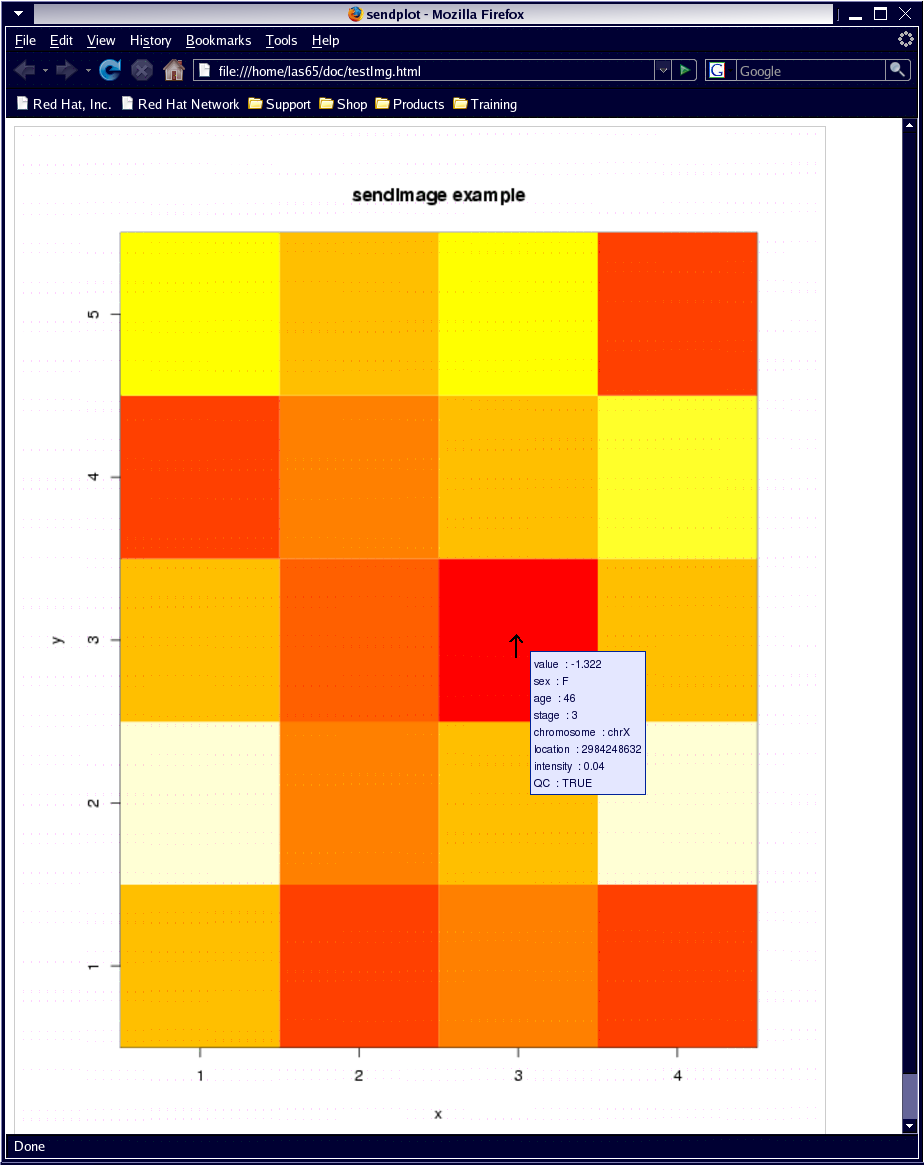
\includegraphics{sendPlotImage}
\caption{A snapshot of our example html file opened in Mozilla Firefox. The information is displayed for the region under the black arrow.}
\end{figure}
\end{center}

\subsection{summary of code used to generate the sendimage example}

 The following is a summary of all code run to make the above example:

\begin{verbatim}
  library("sendplot")

  x = 1:4
  y = 1:5
  z = t(matrix(rnorm(20), ncol=4))

  plot.calls = "image(x=x, y=y, z=z);title(main='sendimage example')"

  x.lbls = list()
  x.lbls$sex = c("F", "M", "F", "F")
  x.lbls$age = c(27, 73, 46, 50)
  x.lbls$stage = c(1,1,3,2)
  x.lbls = as.data.frame(x.lbls)
  
  y.lbls = list()
  y.lbls$chromosome = c("chr1", "chr2", "chrX", "chr7", "chrY")
  y.lbls$location = c(92526, 486844000,2984248632,1387071184,3048286585)
  
  xy.lbls = list()
  intensity = matrix(c(-.3,1.0,.3,-.07,-.4,1.2,.4,.3,1.0,-.5,-.06,1.1,
                       .04,.5,.03,-.09,-.04,.06,.01,.03),nrow=5)
  xy.lbls$intensity = intensity
  QC = matrix(c(T,T,T,T,T,F,T,T,T,F,T,T,T,T,T,F,T,F,T,T), nrow=5)
  xy.lbls$QC = QC

  # automatic detection bound points

  sendimage(plot.call = plot.calls, x=x, y=y, z=z,z.value='value',
            x.lbls = x.lbls, y.lbls=y.lbls, xy.lbls=xy.lbls,
            up.left=c(89,100),low.right=c(800,900),
            source.plot=NA, 
            fname.root="testImg",
            automap=TRUE, automap.method="mode" )

  # or 

  # manual detection bound points


  sendimage(plot.call = plot.calls, x=x, y=y, z=z,z.value='value',
            x.lbls = x.lbls, y.lbls=y.lbls, xy.lbls=xy.lbls,
            up.left=c(89,100),low.right=c(800,900),
            bound.pt=TRUE, source.plot=NA, paint=TRUE,
            img.prog=NA,fname.root="testImg"  )

  # correct bounding points found (101,99), (735,914)

  sendimage(plot.call = plot.calls, x=x, y=y, z=z,z.value='value',
            x.lbls = x.lbls, y.lbls=y.lbls, xy.lbls=xy.lbls,
            up.left=c(101,99),low.right=c(735,914),
            bound.pt=FALSE, source.plot=NA, paint=FALSE,
            img.prog=NA,fname.root="testImg", spot.radius=10)

\end{verbatim}


Again it is not necessary to specify x.lbls, y.lbls, and xy.lbls. If the user only wishes to display z values in interactive window, all may be NA. Like the following call:

\begin{verbatim}
  sendimage(plot.call = plot.calls, x=x, y=y, z=z,z.value='value',
            up.left=c(101,99),low.right=c(735,914),
            bound.pt=FALSE, source.plot=NA, paint=FALSE,
            img.prog=NA,fname.root="testImg", spot.radius=10)

\end{verbatim}

And there you have it, an interactive image! 

\newpage

\section{heatmap.send: heatmap wrapper}


The sendimage function creates a single interactive image. This is a wrapper connecting the heatmap function of the R stats package with sendplot. The majority of the code for this function is verbatim from the R package stats heatmap function. This function was designed to work as a wrapper to utilize the same functionality and plotting as the heatmap function with sendplot's interactive functionality. Authors of heatmap code used in our code: Andy Liaw, original; R. Gentleman, M. Maechler, W. Huber,revisions. The following is an example function call: 

\begin{verbatim}
     heatmap.send(x,Rowv = NULL,
                  Colv = if (symm) "Rowv" else NULL, 
                  distfun = dist,hclustfun = hclust,
                  reorderfun = function(d,w) reorder(d, w),
                  add.expr,symm = FALSE,
                  revC = identical(Colv,"Rowv"),
                  scale = c("row", "column", "none"),
                  na.rm = TRUE, margins = c(5, 5),
                  ColSideColors,RowSideColors,
                  cexRow = 0.2 +  1/log10(nr),
                  cexCol = 0.2 + 1/log10(nc),
                  labRow = NULL,labCol = NULL,
                  main = NULL,xlab = NULL,ylab = NULL,
                  keep.dendro = FALSE, 
                  verbose = getOption("verbose"),
                  mai.mat=NA, mai.prc=FALSE,
                  z.value="value",
                  x.lbls=NA,y.lbls=NA,xy.lbls=NA,
                  bound.pt = FALSE, source.plot=NA,
                  resize="800x1100",
                  ps.paper="letter",ps.width=8,ps.height=11,
                  fname.root="test",dir="./", header="v2",
                  paint=FALSE, img.prog = NA,
                  up.left=c(288,203),low.right=c(620,940),
                  spot.radius=5, automap=FALSE, automap.method="mode") 
\end{verbatim}

\indent {\bf{Note:}} Most of the arguments in this function are arguments for the stats package function heatmap. We will not go through these arguments. Please refer to heatmap documentation for more information. \newline

For the most part the arguments for heatmap.send are consistent with those for sendimage.


\subsection{specifying the plot call}

The function heatmap.send differs from the previous functions, sendxy and sendimage, in that there is no plot.call argument. The heatmap function in the R stats package takes in a matrix of values, x,  and makes a corresponding image. Consider the following example data corresponding to a 5 x 3 image: 

\begin{verbatim}
x =  matrix(rnorm(15), nrow=5, ncol=3)
\end{verbatim}


\indent mai and mai.prc control the plot margins. If mai is NA (default), the application uses default plot margins. For more information on mai, mai.prc, plt.extras, and header please refer to R help files or to the last section of this vignette (i.e., the sendplot section). \newline


\subsection{specifying the interactive points and tool-tip content}

As with the sendimage function, the argument z.value is text which will be used as the descriptor name in the interactive display. Unlike the sendimage function, this does not correspond to an argument z; for the heatmap.send function z.value describes what the argument x holds. \\

\indent {\bf{Note:}} z.value should not contain any spaces or characters; numbers and letters only.\\

\indent As with the sendxy function, the arguments x.lbls, y.lbls, and xy.lbls control what is displayed in the interactive window when the user hovers the mouse over plot points. The arguments x.lbls and y.lbls refer to data that is specific to the x and y values respectively. x.lbls and y.lbls are data.frames. x.lbls is of the dimension n by m where n is equal to the width of the argument x (Our example 3). y.lbls is of the dimension n by m where n is equal to the length of the argument x (Our example 5). Each row is specific to a certain x or y value and each column is a unique variable or characteristic of x or y respectively.  The first row of the data frames should contain column headers; these names will be used as display names in the interactive window that appears. xy.lbls refers to data that is specific to both x and y location. The function argument xy.lbls is a list of matrices; each matrix should be of the same dimensions as x (Our example 5 x 3).

\indent {\bf{Note:}} the function assumes the data.frame rows are in the same order as they appear in the x argument.  \newline
\indent {\bf{Note:}} x values automatically display in the interactive window. If x.lbls, y.lbls, and xy.lbls are NA, the interactive window will only display z values. \newline

\indent The example will continues without specifying x.lbls, y.lbls, or xy.lbls. Please refer to section 3.2 for an example utilizing these arguments. 


\subsection{creating the PNG image file}

\indent heatmap.send follows the same process as sendxy for creating the PNG image file. Please refer to section 2.3 for details.

\subsection{creating the image map}

\indent heatmap.send follows the same process as sendimage for creating the image map. Please refer to section 3.4 for details.


\indent The heatmap function allows for a few different options including color-coded bars for x and y samples, as well as clustering. The following code creates a schema of colors for samples. 
\begin{verbatim}
# color bars for samples
rcol = c("red", "blue", "yellow", "purple", "blue")
ccol = c("black", "green", "black")
\end{verbatim}


\indent Continuing the current example, the following code is executed:
\begin{verbatim}
  heatmap.send(x, RowSideColors=rcol, ColSideColors=ccol,
               z.value="value",
               bound.pt=TRUE, paint=TRUE,source.plot=NA,
               fname.root="heatmapSendPlot",resize="800x1100",
               up.left=c(89,100),low.right=c(800,900),
	       spot.radius=10)
\end{verbatim}

We have entered dummy values for the up.left and low.right coordinates. Figure 6 contains a screenshot of the example PNG file opened in kolourpaint. According to the information in kolourpaint, the up.left location should be 288,203. Notice the grey mouse is over the upper left blue point for the up.left bounding box. The pixel location is shown on the bottom of the window in the second box from the left. It shows a location of 288,203. If we had checked the low.right coordinate it would read 620,940. To complete the process of generating the heatmap.send output, the heatmap.send function used to create this figure should be rerun with bound.pt=FALSE, paint=FALSE,up.left=c(288,203), and low.right=c(620,940).\newline

\begin{center}
\begin{figure}
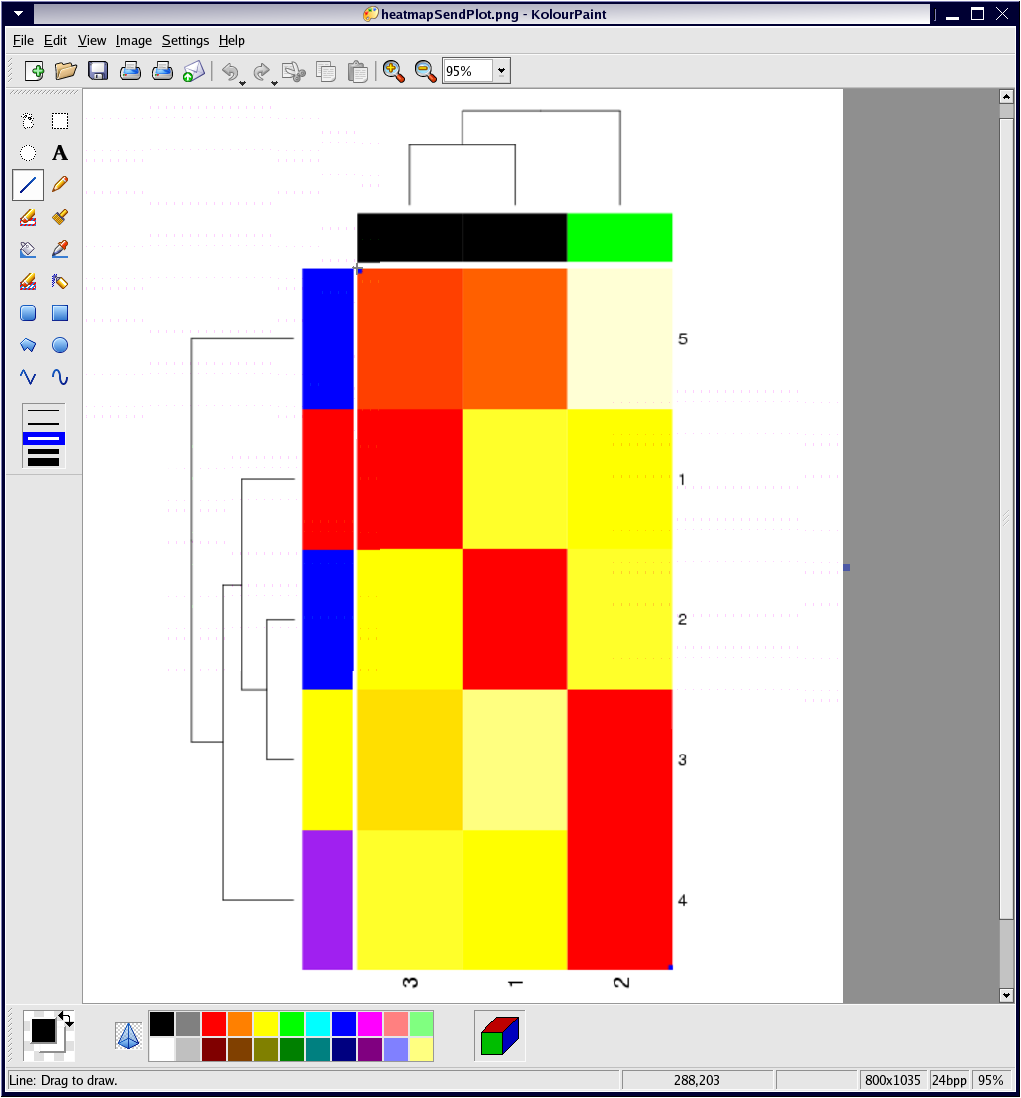
\includegraphics{heatmapPaint}
\caption{A heatmap opened in kolourpaint, showing additional blue points to aid in locating boundaries. Notice where pixel location can be found}
\end{figure}
\end{center}


NOTE: Like the sendxy and sendimage functions, the heatmap.send function does not always need to be run iteratively. If the user is using the same machine (therefore consistent point size and operating system), the plot's xlim, ylim, and margins are the same, and the resize value is the same, the bounding points will also be the same. Helpful hint: setting mai=NA, therefore using the default margins, will keep margins consistent. This process of retrieving bound.pt needs to be performed once for a certain group of settings.\newline

\indent If the automatic detection of bounding points is used, the following code is executed:
\begin{verbatim}
  heatmap.send(x, RowSideColors=rcol, ColSideColors=ccol,
               z.value="value",
               source.plot=NA,
               fname.root="heatmapSendPlot",resize="800x1100",
               up.left=c(89,100),low.right=c(800,900),
	       spot.radius=10, automap=TRUE, automap.method="mode")
\end{verbatim}



\subsection{specifying the spot radius}

\indent The spot.radius argument for heatmap.send is the same as in sendxy. Please refer to section 2.5 for details. 

\subsection{creating the heatmap.send example output}

\indent If automap is used to detect bounding points the function automatically continues making the HTML file and sendxy final example output. 

\indent If bounding points are detected manually, after the correct bounding points are known, the heatmap.send function call should be run again, changing only the up.left, up.right, paint, and bound.pt arguments. up.left and low.right should be updated accordingly. paint and bound.pt should be tripped to FALSE. (NOTE: these are the correct up.left and low.right boundaries when the .png is created from the postscript in linux/unix environment. If the .png file was generated directly the up.left and low.right values of this example may be slightly different).  The following will make the correct interactive plot:
\begin{verbatim}
# manual detection of points

heatmap.send(x, RowSideColors=rcol, ColSideColors=ccol,
             z.value="value",
             bound.pt=FALSE, paint=FALSE,source.plot=NA,
             fname.root="heatmapSendPlot",resize="800x1100",
             up.left=c(288,203),low.right=c(620,940),
	     spot.radius=10)


# or 
# automatic detection of points

heatmap.send(x, RowSideColors=rcol, ColSideColors=ccol,
             z.value="value",
             source.plot=NA,
             fname.root="heatmapSendPlot",resize="800x1100",
             up.left=c(288,203),low.right=c(620,940),
	     spot.radius=10, automap=TRUE,automap.method="mode")

\end{verbatim}


The resulting HTML file may be opened in any web browser that is capable of running Javascript. Figure 7 shows a snapshot of the final graph opened in Mozilla Firefox. Notice how the appropriate information for the region located under the black arrow is displayed in the information box.
\begin{center}
\begin{figure}
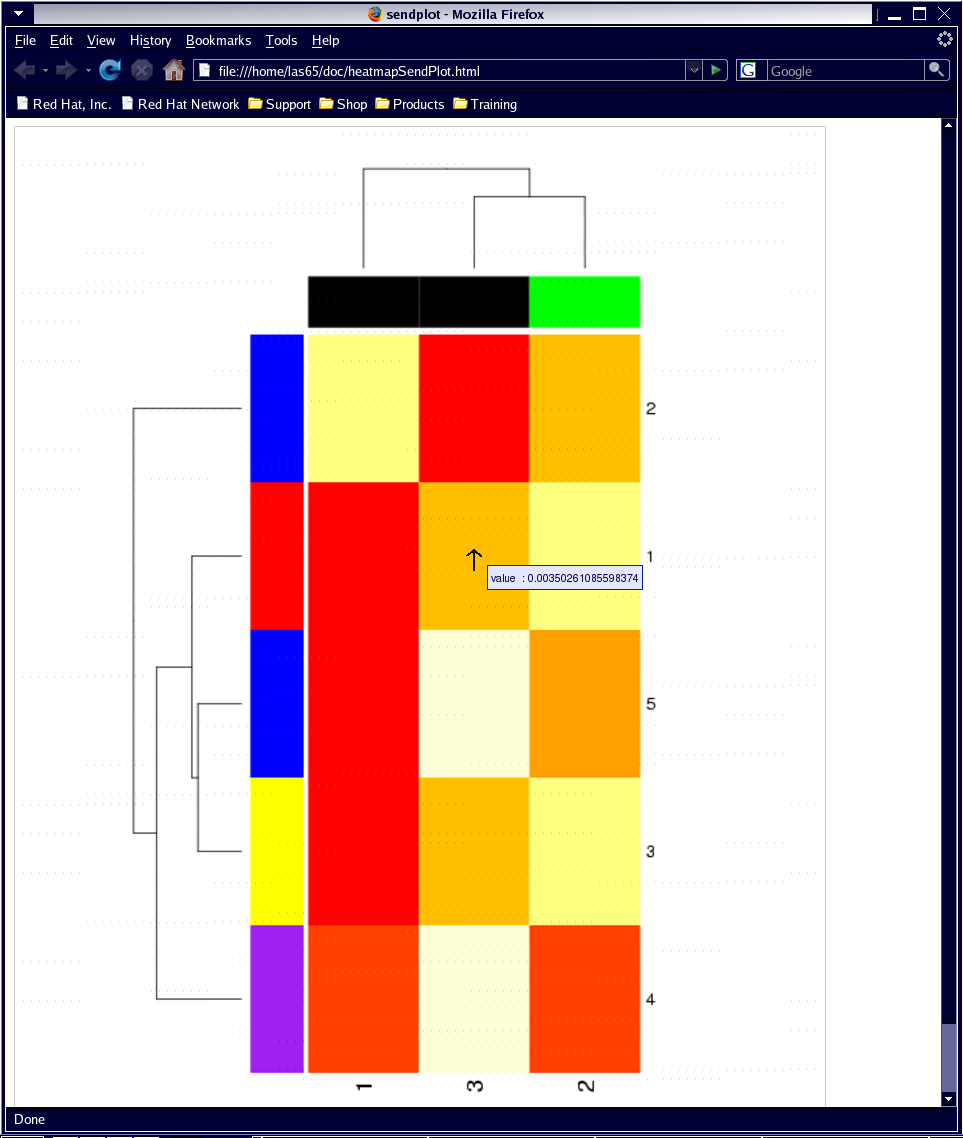
\includegraphics{heatmapFirefox}
\caption{A snapshot of our example HTML file opened in Mozilla Firefox. The information is displayed for the region under the black arrow.}
\end{figure}
\end{center}

\subsection{summary of code used to generate the heatmap.send example}

The following is a summary of all code run to make the above example:

\begin{verbatim}
library("sendplot")
x = matrix(rnorm(15), nrow=5, ncol=3)
rcol = c("red", "blue", "yellow", "purple", "blue")
ccol = c("black", "green", "black")


# automatic detection of bound points
heatmap.send(x, RowSideColors=rcol, ColSideColors=ccol,
              z.value="value",
              source.plot=NA,
              fname.root="heatmapSendPlot",resize="800x1100",
              up.left=c(89,100),low.right=c(800,900),
	      spot.radius=10,automap=TRUE,automap.method="mode")

# or 

# manual detection bound points
heatmap.send(x, RowSideColors=rcol, ColSideColors=ccol,
              z.value="value",
              bound.pt=TRUE, paint=TRUE,source.plot=NA,
              fname.root="heatmapSendPlot",resize="800x1100",
              up.left=c(89,100),low.right=c(800,900),
	      spot.radius=10)

# correct bounding points found (288,203), (620,940)

heatmap.send(x, RowSideColors=rcol, ColSideColors=ccol,
             z.value="value",
             bound.pt=FALSE, paint=FALSE,source.plot=NA,
             fname.root="heatmapSendPlot",resize="800x1100",
             up.left=c(288,203),low.right=c(620,940),
	     spot.radius=10)

\end{verbatim}

As mentioned earlier, the heatmap has options for color bars and for clustering. The code to make the same heatmap without the color bands could be:

\begin{verbatim}
heatmap.send(x, bound.pt=FALSE, paint=FALSE, 
             fname.root="heatmapSendPlot",resize="800x1100",
             up.left=c(288,203),low.right=c(620,940),spot.radius=10)
\end{verbatim}

Or perhaps without the cluster:

\begin{verbatim}
heatmap.send(x,  Rowv=NA, Colv=NA, 
             bound.pt=FALSE, paint=FALSE, 
             fname.root="heatmapSendPlot",resize="800x1100",
             up.left=c(288,203),low.right=c(620,940),spot.radius=10)
\end{verbatim}

These really are just variants of the standard heatmap function. 


And there you have it, an interactive heatmap! 



\newpage


\section{sendplot}

\indent sendplot creates an interactive xy or image plot, additionally displaying any number of decoration plots. The display is governed through the layout. The following is an example function call:
\begin{verbatim}
sendplot <- function(mat, plot.calls, x,y, mai.mat, mai.prc=FALSE,xlim=NA, ylim=NA,
                     z=NA, z.value="value",type="scatterplot", plt.extras = NA,
                     x.lbls=NA, y.lbls=NA, xy.lbls=NA,
                     bound.pt = FALSE,source.plot=NA,resize="4000x5500", 
                     ps.paper="letter", ps.width=8,ps.height=11,
                     fname.root="test",dir="./",header="v2",
                     paint=FALSE,  img.prog = NA,
                     up.left=c(673,715),low.right=c(2874,4481),
                     spot.radius=5,automap=FALSE, automap.method="mode"
                     )
\end{verbatim}

\indent The example code throughout this section will create Figure 8, which displays an interactive heatmap image. 
\begin{center}
\begin{figure}
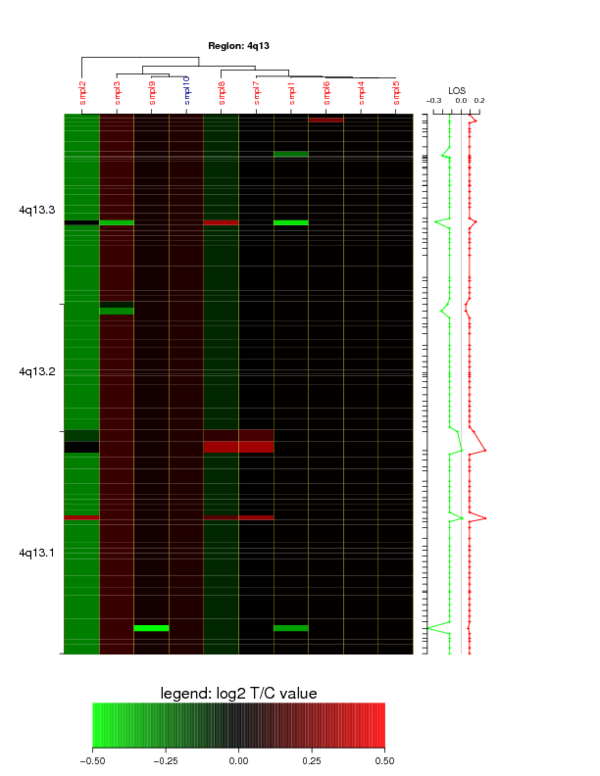
\includegraphics{test}
\caption{Interactive heatmap image}
\end{figure}
\end{center}

\indent {\bf{Note:}} This example utilizes objects created with the R package aCGHplus. aCGHplus is a package designed for array comparative genomic hybridization experiments. For information on this package and objects that can be created with this package, please go to the website: \\http://sphhp.buffalo.edu/biostat/research/software/acghplus/index

\indent Begin by loading the library and example dataset:

\begin{verbatim}
  library(sendplot)
  data("aCGHex")
\end{verbatim}



\subsection{specifying the plot call}

This section will define the following sendplot arguments:

\begin{description}
   \item{mat:~}{numeric matrix governing plot layout}
   \item{plot.calls:~}{character vector of desired plot calls}
   \item{mai.mat:~}{numeric matrix indicating plot margins}
   \item{mai.prc:~}{logical indicating if mai.mat is a percentage of default settings}
   \item{plt.extras:~}{character vector of additional plotting}
\end{description}


\indent The first argument of the sendplot function, mat, is a numeric matrix that is passed into the R graphics package function layout. The first figure, designated '1' in the matrix, is the interactive plot. All other designations represent additional decorative plots of varying complexity. \\
\indent The example (refer to figure 8) contains four different plots. The following creates a layout matrix for the four plots:

\begin{verbatim}
mat=matrix(c(rep(c(rep(2,8),rep(0,2)),1),
       rep(c(rep(1,8),rep(4,2)),14),
       rep(c(rep(3,8),rep(0,2)),2)),
       ncol=10,byrow=TRUE)
\end{verbatim}

\indent This results in the following matrix:

\begin{Schunk}
\begin{Soutput}
      [,1] [,2] [,3] [,4] [,5] [,6] [,7] [,8] [,9] [,10]
 [1,]    2    2    2    2    2    2    2    2    0     0
 [2,]    1    1    1    1    1    1    1    1    4     4
 [3,]    1    1    1    1    1    1    1    1    4     4
 [4,]    1    1    1    1    1    1    1    1    4     4
 [5,]    1    1    1    1    1    1    1    1    4     4
 [6,]    1    1    1    1    1    1    1    1    4     4
 [7,]    1    1    1    1    1    1    1    1    4     4
 [8,]    1    1    1    1    1    1    1    1    4     4
 [9,]    1    1    1    1    1    1    1    1    4     4
[10,]    1    1    1    1    1    1    1    1    4     4
[11,]    1    1    1    1    1    1    1    1    4     4
[12,]    1    1    1    1    1    1    1    1    4     4
[13,]    1    1    1    1    1    1    1    1    4     4
[14,]    1    1    1    1    1    1    1    1    4     4
[15,]    1    1    1    1    1    1    1    1    4     4
[16,]    3    3    3    3    3    3    3    3    0     0
[17,]    3    3    3    3    3    3    3    3    0     0
\end{Soutput}
\end{Schunk}

\indent {\bf{Note:}} In layout, zero acts as a region in which no graph is displayed, a buffer. Notice the use of zero to allow the first and fourth plot to line up in the example.

\indent Figure 9 displays a box version of the above layout.
\begin{center}
\begin{figure}

\includegraphics{layoutFile}
\caption{box display of layout}
\end{figure}
\end{center}


\indent The plot.calls argument is a character vector containing the desired plot calls for all graphs. The first character string must be the call for the interactive plot; this must be either a scatter-plot or an image. For example, the plot.calls argument for Figure 8 is of length four: 


\begin{verbatim}
plot.calls = c(
     "image(x=x,y=y,z=t(z),zlim=c(-0.5,0.5), ylim=range(scanLoc,na.rm=T),
            col=c(hsv(h=2/6,v=seq(1,0,length=1000)^1.15),
            hsv(h=0/6,v=seq(0,1,length=1000)^1.15)),axes=F,xlab='',ylab='')",

     "plot(ddr,axes = FALSE, xaxs = 'i', leaflab = 'none',main=ttl)",

     "image(x=seq(from=-0.5,to=0.5,length=1000),y=1,z=t(zlgnd),zlim=c(-0.5,0.5),
            col=c(hsv(h=2/6,v=seq(1,0,length=1000)^1.15),
                  hsv(h=0/6,v=seq(0,1,length=1000)^1.15)),
            axes=F,xlab='',ylab='')",

     "image(x=0:1,y=0:1,z=matrix(rep(NA,4),ncol=2),xlim=range(c(W.lw,W.up),na.rm=T),
            ylim=range(scanLoc,na.rm=T),zlim=c(0,1),axes=F,xlab='',ylab='')")

\end{verbatim}


\indent The first plot call (given below) creates a heatmap image that looks like Figure 10. 
\begin{verbatim}
"image(x=x,y=y,z=t(z),zlim=c(-0.5,0.5), ylim=range(scanLoc,na.rm=T),
            col=c(hsv(h=2/6,v=seq(1,0,length=1000)^1.15),
            hsv(h=0/6,v=seq(0,1,length=1000)^1.15)),axes=F,xlab='',ylab='')",
\end{verbatim}
 
\begin{center}
\begin{figure}
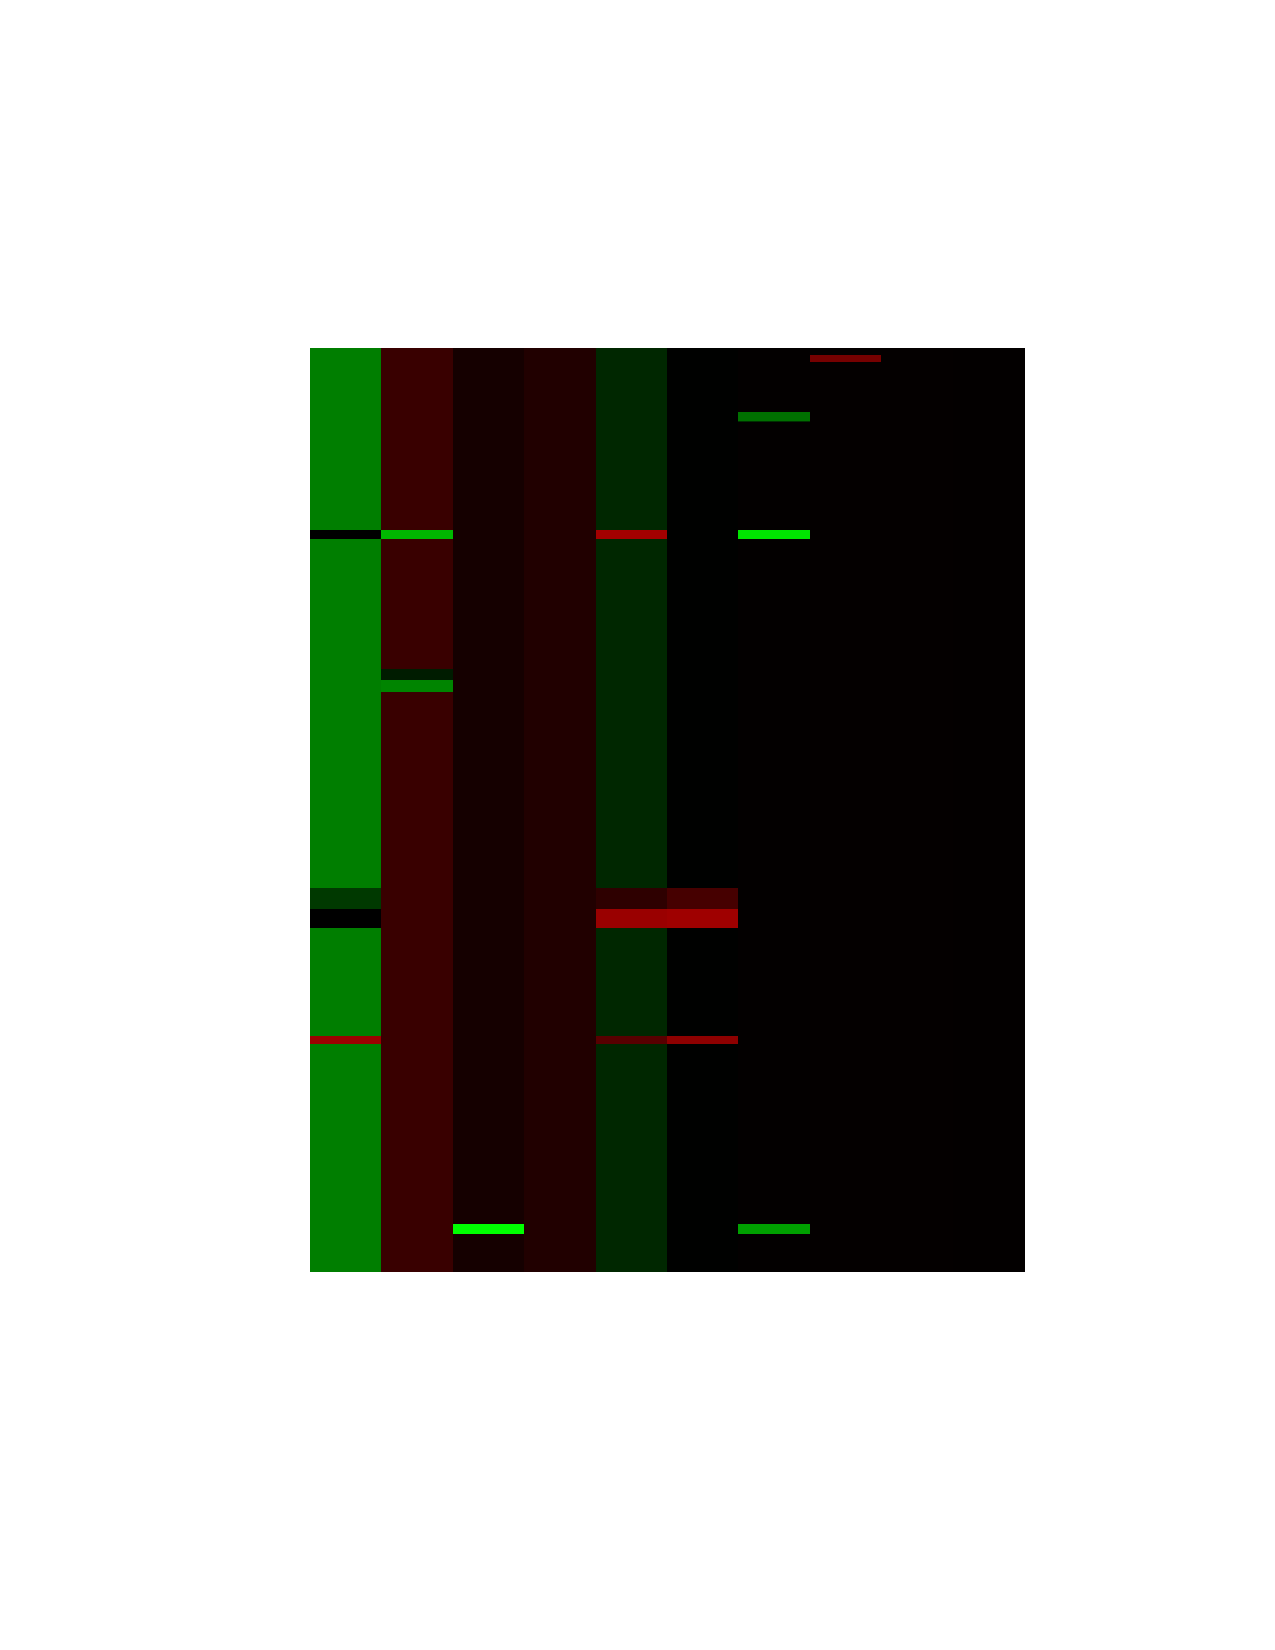
\includegraphics[scale=.5]{heatmap}
\caption{Initial heatmap image from executing plot.call[1]}
\end{figure}
\end{center}

\indent The second plot call (given below) creates the dendrogram representation of sample clustering seen in Figure 11.
\begin{verbatim}
plot(ddr,axes = FALSE, xaxs = 'i', leaflab = 'none',main=ttl)
\end{verbatim}

\begin{center}
\begin{figure}
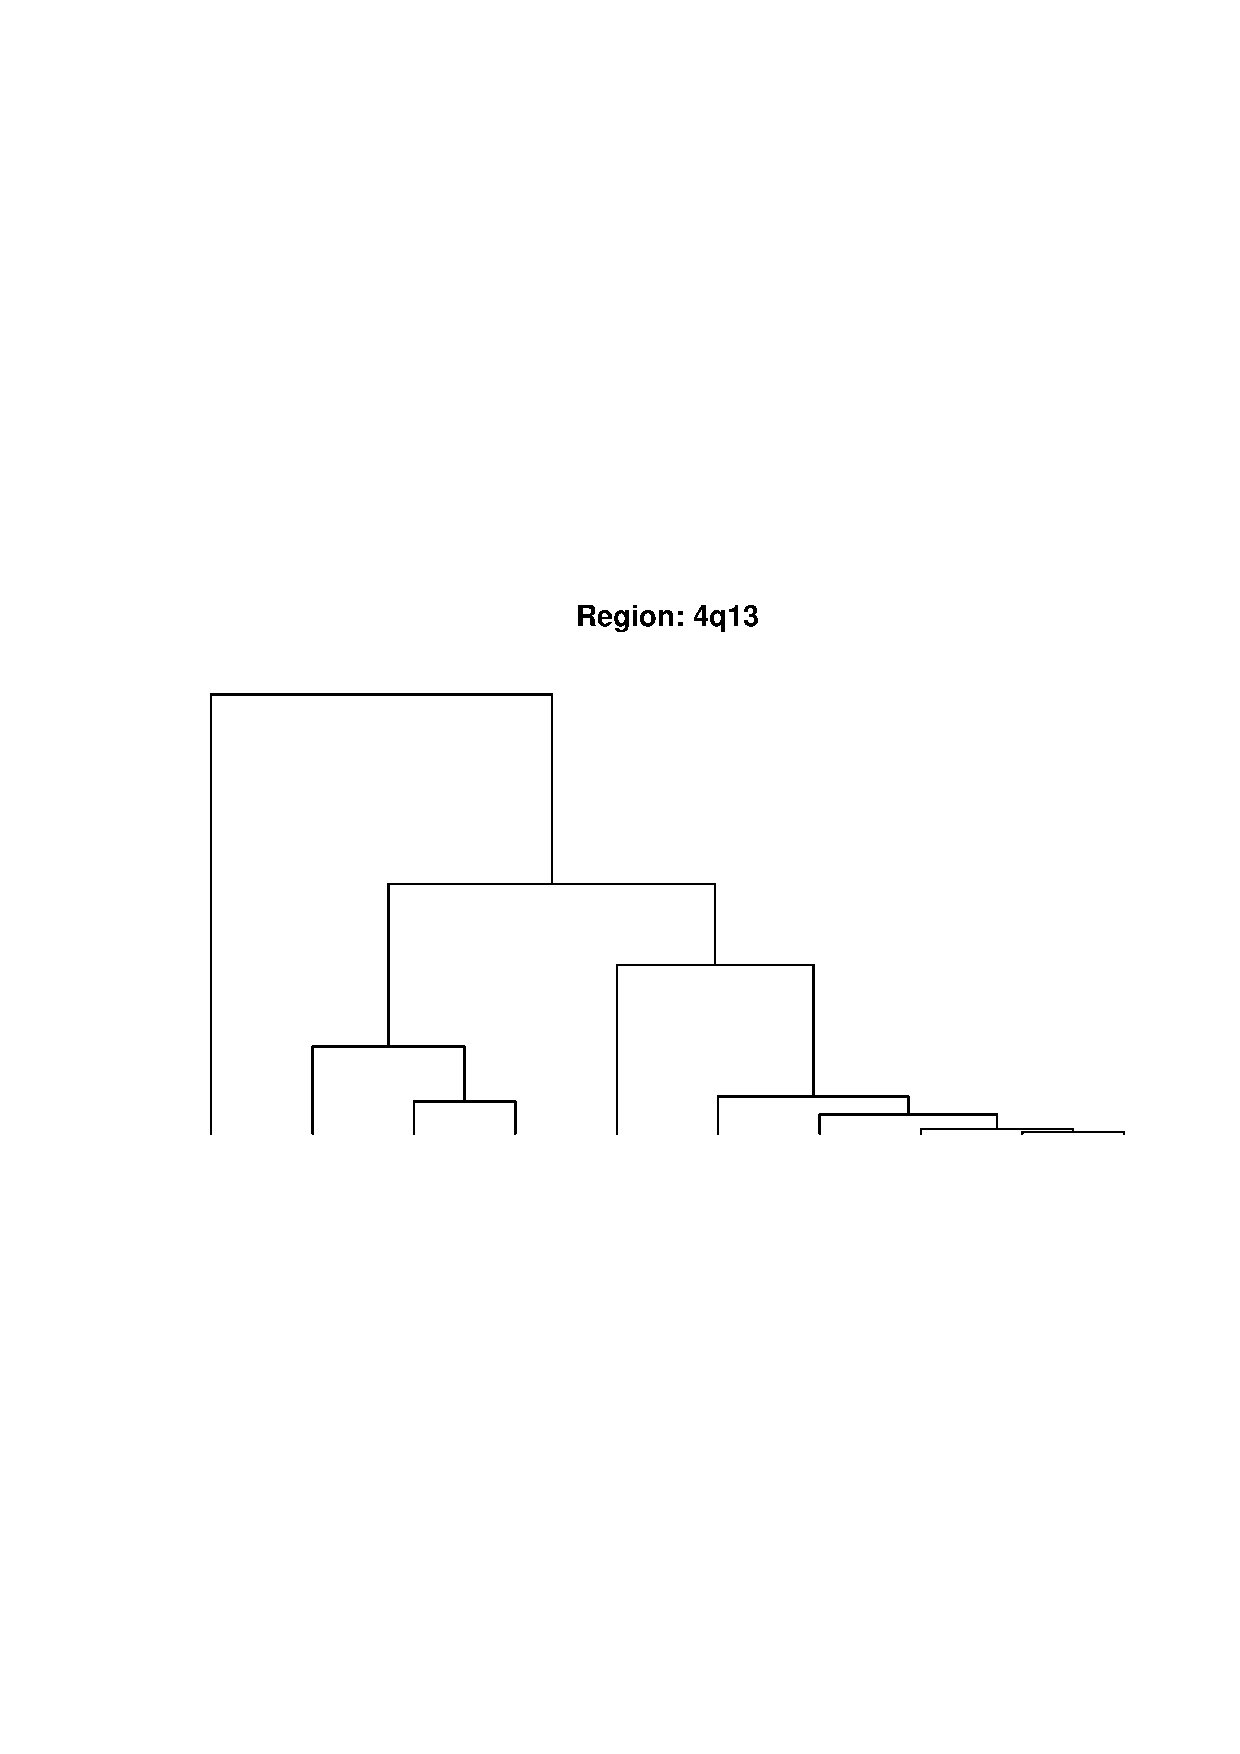
\includegraphics{dendro}
\caption{Dendrogram created from executing plot.call[2]}
\end{figure}
\end{center}

\indent The third plot call, given by:
\begin{verbatim}
  image(x=seq(from=-0.5,to=0.5,length=1000),y=1,z=t(zlgnd),zlim=c(-0.5,0.5),
        col=c(hsv(h=2/6,v=seq(1,0,length=1000)^1.15),
        hsv(h=0/6,v=seq(0,1,length=1000)^1.15)),
        axes=F,xlab='',ylab='')
\end{verbatim}
creates the legend image seen in Figure 12. 
\begin{center}
\begin{figure}

\includegraphics{legend}
\caption{Legend created from executing plot.call[3]}
\end{figure}
\end{center}

\indent The last plot.call, given by: 
\begin{verbatim}
image(x=0:1,y=0:1,z=matrix(rep(NA,4),ncol=2),
        xlim=range(c(W.lw,W.up),na.rm=T),
        ylim=range(scanLoc,na.rm=T),
        zlim=c(0,1),
        axes=F,xlab='',ylab='')
\end{verbatim}
creates a blank image. 

\indent {\bf{Note:}}  The plot call in R adds an automatic buffer that may alter alignment. For this reason  an image call is used for the fourth plot instead of a plot call to ensure ratios and buffers would be equivalent between the first and fourth plots. 

\indent {\bf{Note:}} Notice axis and additional plotting such as vertical line breaks have not yet been plotted. Additional expressions, such as these, can be evaluated on the plots through the sendplot argument plt.extras, which will be discussed in detail later in this section. \newline

\indent Arguments of type character within any of the character strings are specified with a single quotation rather than the double quotations used originally, or vice versa (see second string's leaflab argument). Any variables used in plot calls should be in local memory before running the sendplot function. The following code initializes variables needed for above plot calls:
\begin{verbatim}
# index of genome - we want to look at region 4q13 
# the aCGHplus object has already been subset for this region for 10 samples
   scanDX = 1:dim(aCGH$mapping.info)[1]
   bioDX = scanDX
   scanLoc=aCGH$mapping.info$loc.genome[scanDX]
   scanLoc[which(diff(scanLoc)<=0)]=scanLoc[which(diff(scanLoc)<=0)]-0.001
# add sample names to index of log2 data
   colnames(aCGH$log2.ratios.fitted)=aCGH$inventory$sample.ID
# perform a sample clustering and create dendrogram 
   ManDist=dist(t(aCGH$log2.ratios.fitted),method = "manhattan")
   hc=hclust(ManDist,method="ward")
   ddr=as.dendrogram(hc)
# useful sample information
   nsmpl = aCGH$data.info$nsmpl
   smplDX = 1:nsmpl
   ttl = "Region: 4q13"
# creates legend scale for log2 ratios from -.5 to .5
   zlgnd=array(seq(from=-0.5,to=0.5,length=1000),dim=c(1,1000))
# x values = samples 
   x = 1:length(smplDX)
# y values = genomic location
   y = scanLoc
# z values = log 2 ratios that have been fitted 
# by circular binary segmentation - min and max cutoffs applied
   z.value="log2.ratios.fitted"
   z = aCGH$log2.ratios.fitted[,hc$order]
   z.raw = z
   z[z>0.5]=0.5
   z[z<(-0.5)]=-0.5
# sorts log2 values and splits into low region and high region
# to create fourth plot of avg. means 
   rowSort=function(i,x) sort(x[i,])
   z.sort=t(mapply(rowSort,1:(dim(z.raw)[1]),MoreArgs=list(x=z.raw)))
   lwDX=1:ceiling(nsmpl/4)
   upDX=(floor((3/4)*nsmpl)+1):nsmpl
   W.up=rowMeans(z.sort[,upDX],na.rm=T)
   W.lw=rowMeans(z.sort[,lwDX],na.rm=T)
\end{verbatim}



\indent The sendplot arguments mai.mat and mai.prc control the margins for each plot in the display. The mai.mat argument is a numeric n x 4 matrix, where n is the length of plot calls. Each row of mai.mat is passed into the R graphics package function par specifying mai. The four columns represent the margins: bottom, left, top, and right respectively. The first row corresponds to the margins for layout designates '1', the second row to layout designates '2' and so forth. If the numeric values in the mai.mat represent a percentage of the default margins, the argument mai.prc=TRUE. The following sets up margins for Figure 8:
\begin{verbatim}
mai.mat = matrix(0, ncol=4, nrow=4, byrow=TRUE)
mai.mat[1,] = c(.5,0,.5,0)
mai.mat[2,] = c(0,0,.3,0)
mai.mat[3,] = c(.4,.4,.2,.4)
mai.mat[4,] = c(.5,.2,.5,.2)
mai.prc = FALSE
\end{verbatim}



\indent {\bf{Note:}} If figure margins are too large, an error will occur when plotting.  If the user gets an error message like 'Error figure margins too large', try decreasing the values in mai.mat.


\indent plt.extras contains additional expressions or plot calls for each displayed plot. plt.extras is a list which contains sub-lists corresponding to each plot in plot.calls. Each of these sub-lists is a list of character strings to be evaluated as R functions. Before examining the plt.extra calls for Figure 8, consider the following smaller example: The desired display has two plots. The first plot requires the additional plotting of a vertical line at y=0 and a title while the second requires no additional plotting.

\begin{verbatim}
plt.extras = list()
plt.extras$plot1 = NA
test = list()
test[1] = "abline(v=0, col='gray77', lwd=1)"
test[2] = "title(main='mytest')"
plt.extras$plot2 = test
\end{verbatim}  

\indent Notice arguments of type character within any of the character strings are specified with a single quotation rather than the double quotations used originally, or vice versa (see col argument).

\indent Now looking back at Figure 8 compared with Figure 10, additional axes on the top and left with labels, as well as vertical lines to separate x-values are desired. The following code will achieve this:  

\begin{verbatim}
plot1 = list()
plt1.ind = 1

nlbl=50
eval.js("sample.colors=as.character(aCGH$inventory$sex)")
colorSet =c("hotpink","darkblue", "green")
lev = levels(factor(sample.colors))
for(i in 1:length(lev)){
  sample.colors[sample.colors==lev[i]] = colorSet[i]
}
count.arm=sum((aCGH$Band.Aid$Regions[[2]]$Upper>=min(scanLoc,na.rm=T))
  &(aCGH$Band.Aid$Regions[[2]]$Lower<=max(scanLoc,na.rm=T)))
count.broadband=sum((aCGH$Band.Aid$Regions[[3]]$Upper>=min(scanLoc,na.rm=T))
  &(aCGH$Band.Aid$Regions[[3]]$Lower<=max(scanLoc,na.rm=T)))
count.finband=sum((aCGH$Band.Aid$Regions[[4]]$Upper>=min(scanLoc,na.rm=T))
  &(aCGH$Band.Aid$Regions[[4]]$Lower<=max(scanLoc,na.rm=T)))
cat("label counts:",count.arm,count.broadband,count.finband,fill=T)
cat("target number=",nlbl,fill=T)
ilbl=order(abs(c(count.arm,count.broadband,count.finband,length(scanDX))-nlbl))[1]
cat("ilbl=",ilbl,fill=T)
if(ilbl<=3){
  if(ilbl==1) bandDX=1:40
  if(ilbl==2) bandDX=(
       (sum(aCGH$Band.Aid$Regions[[3]]$Upper<=min(scanLoc,na.rm=T),na.rm=T)+1)
       :(sum(aCGH$Band.Aid$Regions[[3]]$Lower<=max(scanLoc,na.rm=T),na.rm=T)))
  if(ilbl==3) bandDX=(
       (sum(aCGH$Band.Aid$Regions[[4]]$Upper<=min(scanLoc,na.rm=T),na.rm=T)+1)
       :(sum(aCGH$Band.Aid$Regions[[4]]$Lower<=max(scanLoc,na.rm=T),na.rm=T)))
  lbls=paste(aCGH$Band.Aid$Regions[[ilbl+1]]$Chrom[bandDX],
    aCGH$Band.Aid$Regions[[ilbl+1]]$Label[bandDX],sep="")


  plot1[plt1.ind] =  "axis(2,aCGH$Band.Aid$Regions[[ilbl+1]]$Center[bandDX],
                           tick=F,labels=lbls,las=2,cex.axis=1)"
  plt1.ind = plt1.ind +1 
  plot1[plt1.ind] = "axis(2,aCGH$Band.Aid$Regions[[ilbl+1]]$Lower[bandDX], labels=F)"
  plt1.ind = plt1.ind +1 
  
}
if(ilbl==4){   
  lbls=as.character(aCGH$mapping.info$spot.ID[scanDX])

  plot1[plt1.ind] = "axis(2,aCGH$mapping.info$loc.genome[scanDX],tick=F,
          labels=lbls, las=2,cex.axis=1)"
  plt1.ind = plt1.ind +1 
}

plot1[plt1.ind] = "abline(v=(0:nsmpl)+1/2,col=7,lty=1,lwd=1/3)"
plt1.ind = plt1.ind +1


if(length(sample.colors)==1){

  plot1[plt1.ind] = "axis(3,1:length(smplDX),cex.axis=1,las=2,
                     labels=aCGHsub$inventory$sample.ID[hc$order])"
  plt1.ind = plt1.ind +1 
}                                      
if(length(sample.colors)!=1){
  unq.colors=unique(sample.colors[hc$order])
  lbls2=aCGH$inventory$sample.ID[hc$order]
  col.labs=sample.colors[hc$order]
  for(j in 1:length(unq.colors)){
    iclr = unq.colors[j]
    cat("eye color=",iclr,fill=T)
    nm = paste("adx",j,sep="")
    eval.js(paste(nm, "=which(col.labs==iclr)",sep=""))

    plot1[plt1.ind] = paste("axis(3,",nm,",labels=lbls2[",nm,"],
                      cex.axis=1,las=2,col.axis='",iclr,"')", sep="")
    plt1.ind = plt1.ind +1 
  }     
}
\end{verbatim}




\indent The second plot, Figure 11 of the  dendrogram, does not require any additional plotting and is set as NA. The legend created by the third plot call (Figure 12) requires a title and bottom axis. This is achieved with the following:

\begin{verbatim}
plot3 = list()
plt3.ind = 1

plot3[plt3.ind] = "mtext('legend: log2 T/C value',side=3,cex=1,line=1/4)"
plt3.ind = plt3.ind + 1
plot3[plt3.ind] = "axis(1,seq(from=-0.5,to=0.5,length=5),line=0)"
plt3.ind = plt3.ind + 1
\end{verbatim}



\indent The fourth graph still needs to be generated since we only set up a blank image. The following calls create the fourth plot:

\begin{verbatim}
plot4 = list()
plt4.ind = 1

plot4[plt4.ind] = "abline(v=0,col='gray77',lwd=1)"
plt4.ind = plt4.ind + 1
plot4[plt4.ind] = "points(W.lw,scanLoc,col='green',pch=3,cex=0.5)"
plt4.ind = plt4.ind + 1
plot4[plt4.ind] = "points(W.up,scanLoc,col='red',pch=3,cex=0.5)"
plt4.ind = plt4.ind + 1
plot4[plt4.ind] = "lines(W.lw,scanLoc,col='green',pch=3,cex=0.5)"
plt4.ind = plt4.ind + 1
plot4[plt4.ind] = "lines(W.up,scanLoc,col='red',pch=3,cex=0.5)"
plt4.ind = plt4.ind + 1
plot4[plt4.ind] = "axis(3)"
plt4.ind = plt4.ind + 1
plot4[plt4.ind] = "mtext(text='LOS',side=3,line=2,cex=0.5)"
plt4.ind = plt4.ind + 1
plot4[plt4.ind] = "axis(2,at=scanLoc,labels=F)"
plt4.ind = plt4.ind + 1
\end{verbatim}


\indent Now the above code chunks generate all the sub-lists of the plt.extras list. The following will put all the sub-lists in the plt.extras list object:

\begin{verbatim}
plt.extras = list()
plt.extras$plot1 = plot1
plt.extras$plot2 = NA
plt.extras$plot3 = plot3
plt.extras$plot4 = plot4
\end{verbatim}



\indent  Notice how plt.extras adds any additional plot calls to the original plots. Looking at the third plot's sub-list, there are two additional calls: one to make the title and another to make the axis. 

\begin{Schunk}
\begin{Sinput}
> plot3
\end{Sinput}
\begin{Soutput}
[[1]]
[1] "mtext('legend: log2 T/C value',side=3,cex=1,line=1/4)"

[[2]]
[1] "axis(1,seq(from=-0.5,to=0.5,length=5),line=0)"
\end{Soutput}
\end{Schunk}


\indent {\bf{Note:}} Some of the plt.extras argument can be included in the original plot.calls argument. The original character string can contain multiple calls separated by a semicolon. For example, the third plot.call for the heatmap legend original is the following:
  
\begin{verbatim}
"image(x=seq(from=-0.5,to=0.5,length=1000),y=1,z=t(zlgnd),zlim=c(-0.5,0.5),
            col=c(hsv(h=2/6,v=seq(1,0,length=1000)^1.15),
                  hsv(h=0/6,v=seq(0,1,length=1000)^1.15)),
            axes=F,xlab='',ylab='')",
\end{verbatim}

The plt.extras calls for this image are: 
\begin{verbatim}
  "mtext('legend: log2 T/C value',side=3,cex=1,line=1/4)"
  
   and 

   "axis(1,seq(from=-0.5,to=0.5,length=5),line=0)"
\end{verbatim}


\indent These could have been combined thus changing the plt.extra call to NA and the plot.call to:
\begin{verbatim}
"image(x=seq(from=-0.5,to=0.5,length=1000),y=1,z=t(zlgnd),zlim=c(-0.5,0.5),
            col=c(hsv(h=2/6,v=seq(1,0,length=1000)^1.15),
                  hsv(h=0/6,v=seq(0,1,length=1000)^1.15)),
            axes=F,xlab='',ylab=''); 
            mtext('legend: log2 T/C value',side=3,cex=1,line=1/4);
            axis(1,seq(from=-0.5,to=0.5,length=5),line=0)"
\end{verbatim}


\subsection{specifying the interactive points and tool-tip content}


\indent The currently supported graph types for the interactive plot are scatterplot and image. The arguments x, y, z, z.value, xlim, ylim, x.lbls, y.lbls, xy.lbls and type are defined differently depending on which interactive plot is used. \\
\indent The sendplot argument type refers to which supported graph type is the interactive plot. type should either be 'scatterplot' or 'image'.

\subsubsection{scatterplot}

\indent The x and y arguments are the x and y coordinates of desired interactive points. z and z.value are not utilized and should be left as default values (NA). 

\indent If the first plot is a scatterplot, no xlim or ylim value should be specified in the first plot.call. For mapping purposes, xlim and ylim must be given as separate arguments to the sendplot function. If xlim and ylim are not set in the arguments, or entered as NA, the range of the x and y values will be used.

\indent The arguments x.lbls, y.lbls, and xy.lbls control what is displayed in the interactive window when the user hovers the mouse over plot points. The arguments x.lbls and y.lbls refer to data that is specific to the x and y values respectively. The argument xy.lbls governs data specific to both x and y location. In the case of a scatter-plot, x.lbls, y.lbls, and xy.lbls refer to the same position; it is only necessary to use either x.lbls or y.lbls. x.lbls and y.lbls are data.frames with the number of rows equal to the number of interactive data points. The first row of the data frame should contain column headers; these names will be used as display names in the interactive window that appears. \newline

\indent {\bf{Note:}} Please refer to section 2.2 for more details. 

\subsubsection{image}

\indent The x, y, and z arguments are the x, y, and z used in the image call. x and y are the locations of the grid lines at which the values of z correspond. z is a matrix of values (length of x  by length of y).  These three arguments have already been defined for the example in the previous section. The function argument z.value describes what z holds (examples pvalues, logRatios, percentAccepted); this identifier is used in the interactive display. The data being used as z values for Figure 8 are log2 ratios that have been fitted by circular binary segmentation. We will call our z.value log2ratios.fitted.

\begin{verbatim}
z.value = "log2ratios.fitted"
xlim = NA
ylim = NA
type = "image" 
\end{verbatim}



\indent {\bf{Note:}} z.value should not contain any spaces or punctuation characters; numbers and letters only. \newline

\indent Notice in the above code we have set xlim and ylim as NA. When the interactive plot is an image, these values are generated from the image call. 

\indent As with the scatterplot function, the arguments x.lbls, y.lbls, and xy.lbls control what is displayed in the interactive window when the user hovers the mouse over plot points. The arguments x.lbls and y.lbls refer to data that is specific to the x and y values respectively. x.lbls and y.lbls are data.frames of the dimension n by m, where n is equal to the length of x or y respectively. Each row is specific to a certain x or y value and each column is a unique variable or characteristic of x or y respectively.  The first row of the data frames should contain column headers; these names will be used as display names in the interactive window that appears. The xy.lbls argument is a little different because it governs data specific to both x and y locations. The function argument xy.lbls is a list of matrices; each matrix is of the dimension n by m, where n is equal to the length of y and m is equal to the length of x.\\ 

\indent {\bf{Note:}} the function assumes the data.frame rows are in the same order as they appear in the x argument (or y argument if y.lbls).  \newline

\indent {\bf{Note:}} z values automatically display in the interactive window. If x.lbls, y.lbls, and xy.lbls are NA, the interactive window will only display z values. \newline 

\indent For the example, x-values are samples. We have 43 x-values and therefore 43 rows in the x.lbls data.frame. The sample specific data that is selected for display in the interactive window are sample.IDs and sex. The aCGH object contains a data.frame that holds information about the samples: the first column of that data frame holds the sample.ID information and the eighth column holds the sex data. Earlier we ordered the samples by clustering, this ordering is used for subsetting. The x.lbls data frame may be attained with the following:

\begin{verbatim}
x.lbls=aCGH$inventory[hc$order,c(1,8)]
y.lbls=aCGH$mapping.info[scanDX,c(5,6,8,10,12)]
\end{verbatim}


\indent The y-values for the example are BACs of specific genomic location. A specific range of BACs was selected previously by setting scanDX. scanDX retrieves information for a region of chromosome 4.  There are 98 different y-value locations selected and therefore y.lbls will have 98 rows. The selected y-specific data are genomic location, chromosome, arm, broad.band, and fine.band location in the interactive display. The aCGH object contains a data.frame that holds information about the BACs; the corresponding columns in that data.frame are 5, 6, 8. 10, and 12. \\

\indent The xy specific data desired for display in the interactive window are raw log2 ratios and the log2 ratios that have been fitted by circular binary segmentation. Since the fitted log 2 ratios are used as the z values to create the heatmap, these values are displayed automatically in the interactive window. The xy.lbls list contains information for the raw log2 ratios. 

\begin{verbatim}
xy.lbls=list();
log2.ratio = as.matrix(aCGH$log2.ratios[,hc$order])
xy.lbls$log2.ratio = log2.ratio
\end{verbatim}



\subsection{creating the PNG image file}

\indent sendplot follows the same process as sendxy for creating the PNG image file. Please refer to section 2.3 for details.

 For the example plot, the final image is made smaller in both width and height by the following resize value. \newline

\begin{verbatim}
 resize="600x900"

\end{verbatim}



\subsection{creating the image map}

\indent The sendplot argument header refers to which java tooltip is used in the html file. Older versions of the package utilized a tooltip that worked well with Mozilla Firefox but would not work on Internet Explorer web browsers. header may either be 'v1' or 'v2'. The more recent tooltip ('v2') which is the current default, works on multiple web browsers.\\


As mentioned previously, the sendplot functions output an HTML file and a PNG image. The HTML file contains an image map which identifies the interactive regions of the PNG image (i.e., the regions for which a tool-tip will appear). The image map requires a mapping of the plotted point coordinates as specified in the R plotting calls that generated them to the corresponding pixel location on the final PNG image. The sendplot functions build this map by identifying the upper-left and lower-right locations in the original plotting coordinate system and in the final pixel coordinate system. The function arguments for these coordinates are given as:
\begin{description}
  \item{up.left:~}{The x and y value in pixels of the upper left hand
    corner of the plot call}
  \item{low.right:~}{The x and y value in pixels of the lower right hand
    corner of the plot call.}
\end{description}

\indent The sendplot functions provide convenient options for identifing the upper-left and lower-right pixil coordinates. There is an automatic detection of bounding points, in most cases eliminating the two step procedure. There are also options for manual detection of bound points. These options will be discussed further in the following sections.  

\subsubsection{automatic dectection of bounding points}

\indent As mentioned previously, there is an option for automatic detection of the upper-left and lower-right pixil coordinates. This option eliminates the two iteration procedure for linux and unix users. The functions utilizes ImageMagick's convert program installed on most linux machines, and the R library rtiff's readTiff function. The function arguments implementing this option are:
\begin{description}
 \item{automap:~}{logical indicating if application should
    attempt to automatically detect upper-left and lower-right 
    coordinates.}

  \item{automap.method:~ }{if automap is TRUE, the method that will be
    used to find bound points. The current options are median and mode}

 \end{description}

\indent For windows and mac users, this automatic detection of coordinates is viable if the user has the ability to convert a PNG image to a TIFF image. The current implemenation still requires two iterations. The first iteration will create the PNG images. The user then must manually convert the PNG images to the TIF images using appropriate file names. The function is run again and the auto detect will function correctly.  

\indent Continuing the current example, the following code is executed:
\begin{verbatim}
sendplot(mat=mat, plot.calls=plot.calls, mai.mat=mai.mat,
         x=x,y=y,z=z,xlim=NA,ylim=NA, z.value=z.value, type="image",
         plt.extras=plt.extras, x.lbls=x.lbls, y.lbls=y.lbls,xy.lbls=xy.lbls, 
         spot.radius=3,up.left=c(673,715),low.right=c(2874,4481),
         source.plot=NA, resize=resize,
         automap=TRUE, automap.method="mode")
\end{verbatim}


\subsubsection{manual detection of bounding points}

\indent As mentioned previously, the sendplot functions are typically run in two iterations when creating interactive plots for the first time. In the first iteration, the PNG file is created and then opened in a program such as mspaint or kolourpaint so that the upper-left and lower-right pixel coordinates are identified. In the second iteration, the function is called again using the pixel coordinates identified in the first iteration and the PNG and HTML output files are created.  Refer back to Figure 1 for a flowchart for this two-iteration procedure. 


\indent The sendplot functions  include arguments which allow for the convenient identification of the up.left and low.right values. These arguments are:

\begin{description}
 \item{paint:~}{logical indicating if application should
    automatically open the .png file for the user to view .png file and/or
    to retrieve needed bounding values of the plot call.}

  \item{img.prog:~ }{if paint is TRUE, the command line call that will open
    a program to view .png file to retrieve pixel locations of interactive
    plot bounds. If this is left NA, the operating system is checked and
    a default program is used. For unix the default application is
    kolourpaint and for windows it is microsoft paint (mspaint).}

  \item{bound.pt:~}{logical indicating if red points should be plotted to
    aid in finding the upper left and lower right coordinates. If
    bound.pt is FALSE, indicates that up.left and low.right arguments
    are correct and will make the html file. Note that if bound.pt is TRUE then the function will not
    attempt the task of writing the .html file as that step can be time consuming.}

 \end{description}
One way to identify the up.left and low.right values in the first iteration of sendplot construction is to execute the function with: bound.pt=TRUE, paint=TRUE, and img.prog=NA. With these combination of arguments, the function will create the PNG output, add red points to the upper-left and lower-right corners, and then open the PNG in the default viewer so that the user can readily identify the up.left and low.right pixel coordinates. 

\indent {\bf{Note:}} additional points added to upper-left and lower-right corners are red for scatter-plots and blue for 
images. \newline

 \indent Figure 13 is a snapshot of the sendplot help function example for scatter-plot opened in kolourpaint:

\begin{center}
\begin{figure}
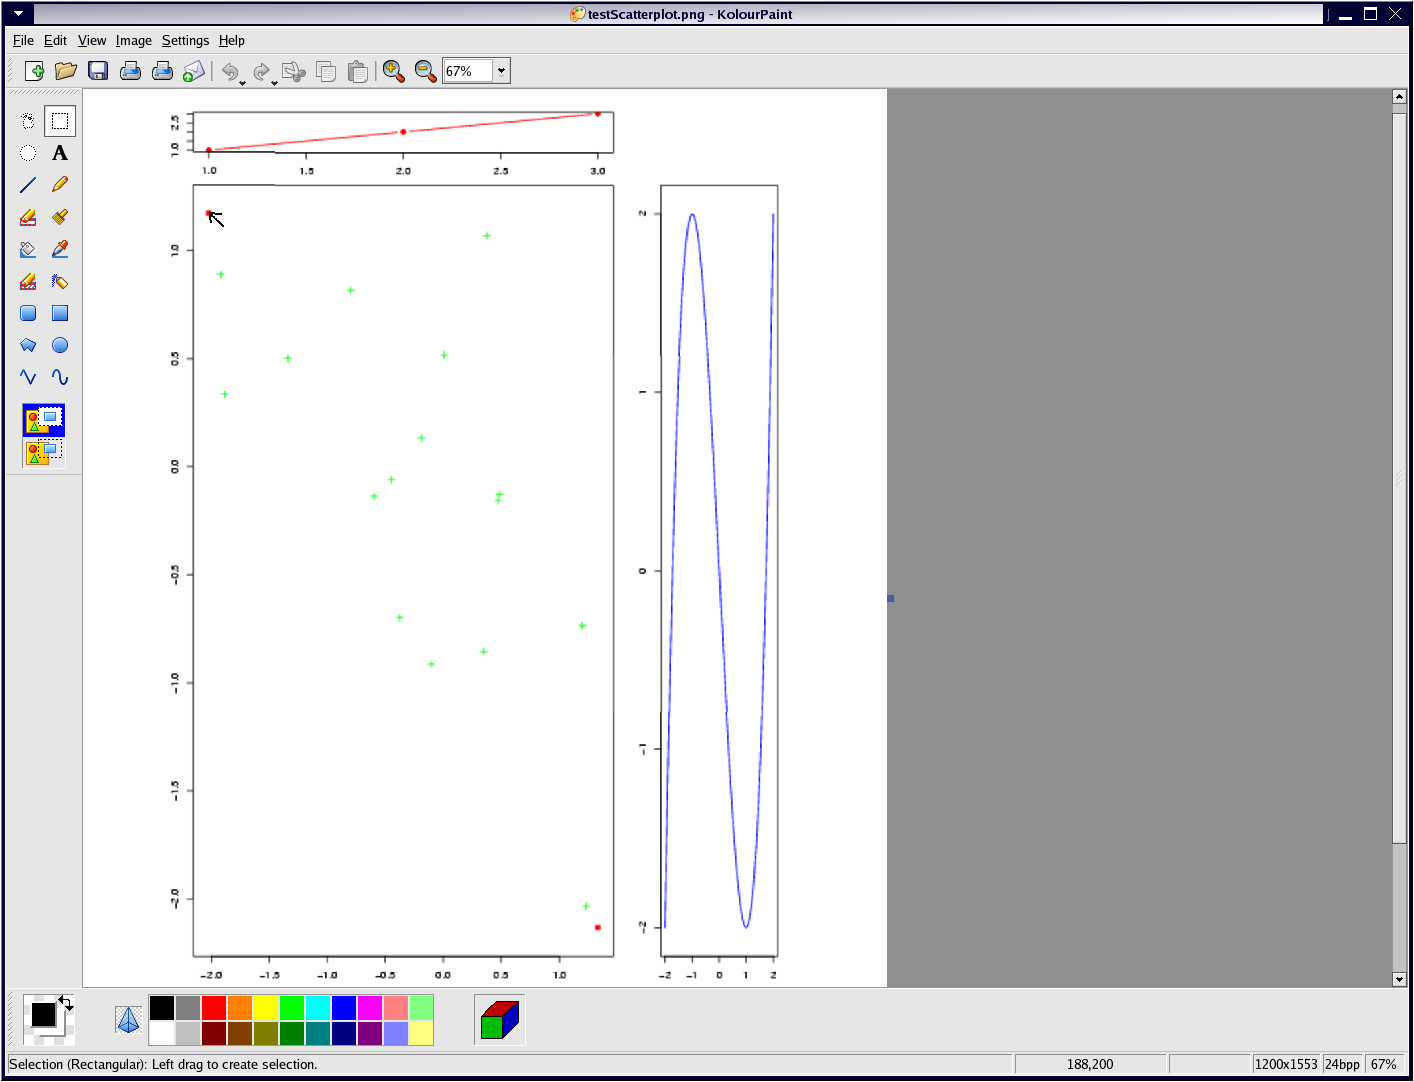
\includegraphics{sendPlot2}
\caption{A scatter-plot opened in kolourpaint, showing additional red points to aid in locating boundaries. Notice where pixel location can be found}
\end{figure}
\end{center}

\indent  Notice the mouse is over the upper left red point for the up.left bounding box. The pixel location is shown on the bottom of the window in the second box from the left. It shows a location of 188, 200. The lower-right corner should also be check and the sendplot function used to generate this plot rerun with bound.pt=FALSE, paint=FALSE, and the corrected up.right and low.left pixel locations. \\

\indent Continuing with the example for Figure 8, the following code is executed:
\begin{verbatim}
sendplot(mat=mat, plot.calls=plot.calls, mai.mat=mai.mat,
         x=x,y=y,z=z,xlim=NA,ylim=NA, z.value=z.value, type="image",
         plt.extras=plt.extras, x.lbls=x.lbls, y.lbls=y.lbls,xy.lbls=xy.lbls, 
         spot.radius=3,up.left=c(673,715),low.right=c(2874,4481),
         source.plot=NA, img.prog=TRUE,
         resize=resize,bound.pt=TRUE, paint=TRUE)
\end{verbatim}
We have entered dummy values for the up.left and low.right coordinates. Figure 14 contains a screenshot of the example PNG file opened in kolourpaint. {\bf{Note:}} We have circled the mouse location in blue to aid in viewing. Your mouse will not have the blue circle surrounding it.\\ \indent  According to the information in kolourpaint, the up.left location should be 83,97. Notice the mouse is over the upper left red point for the up.left bounding box. The pixel location is shown on the bottom of the window in the second box from the left. It shows a location of 83,97. If we had checked the low.right coordinate it would read 430,635. To complete the process of generating the sendplot output, the sendplot function used to created this figure should be rerun with bound.pt=FALSE, paint=FALSE,up.left=c(83,97) and low.right=c(430,635). \newline

\begin{center}
\begin{figure}
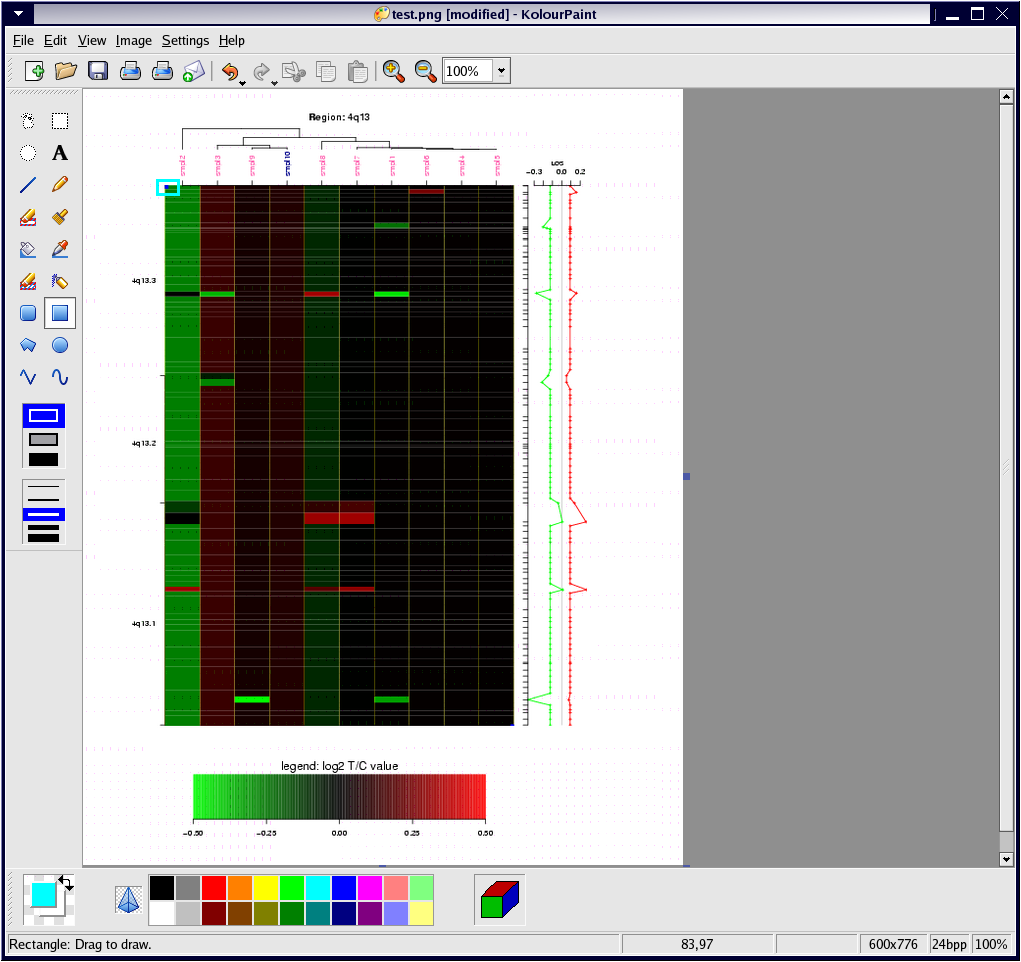
\includegraphics{sendPlot3}
\caption{Our example image opened in kolourpaint. The boundaries of the image is where the pixel location should be taken.}
\end{figure}
\end{center}

NOTE: As mentioned earlier, the sendxy function does not always need to be run iteratively. If the user is using the same machine (therefore consistent point size and operating system), the plot's xlim, ylim, and margins are the same, and the resize value is the same, the bounding points will also be the same. Helpful hint:  In may cases if the user is generating similar plots, the xlim and ylim can be set constant so that all graphs are on the same scale; mai=NA using the default margins will also be consistent. This process of retrieving bound.pt needs to be performed once for a certain group of settings.\newline
\\


\subsection{specifying the spot radius}

\indent The spot.radius argument controls how large an area will be active when the mouse is scrolled over. If the user selects a larger region, some spot locations may overlap and be lost. The interactive application is very sensitive if the user selects a low region. The users' discretion is best used here given that the plot scale and number of data points will also play a role in determining a good spot.radius.  \\


\subsection{creating the sendplot example output}

\indent If automap is used to detect bounding points the function automatically continues making the HTML file and sendxy final example output. 

\indent If bounding points are detected manually, after the correct bounding points are known, the sendplot function call should be run again, changing only the up.left, up.right, paint, and bound.pt arguments. up.left and low.right should be updated accordingly. paint and bound.pt should be tripped to FALSE. (NOTE: these are the correct up.left and low.right boundaries when the .png is created from the postscript in linux/unix environment. If the .png file was generated directly the up.left and low.right values of this example may be slightly different).  The following will make the correct interactive plot:

\begin{verbatim}

# manual detection of points

sendplot(mat=mat, plot.calls=plot.calls, mai.mat=mai.mat,
         x=x,y=y,z=z,xlim=NA,ylim=NA, z.value=z.value, type="image",
         plt.extras=plt.extras, x.lbls=x.lbls, y.lbls=y.lbls,xy.lbls=xy.lbls, 
         spot.radius=3,up.left=c(83,97),low.right=c(430,635),
         source.plot=NA, img.prog=TRUE,
         resize=resize, bound.pt=FALSE, paint=FALSE)

# or 
# automatic detection of points
sendplot(mat=mat, plot.calls=plot.calls, mai.mat=mai.mat,
         x=x,y=y,z=z,xlim=NA,ylim=NA, z.value=z.value, type="image",
         plt.extras=plt.extras, x.lbls=x.lbls, y.lbls=y.lbls,xy.lbls=xy.lbls, 
         spot.radius=3,up.left=c(83,97),low.right=c(430,635),
         source.plot=NA,resize=resize,
	 automap=TRUE, automap.method="mode")



\end{verbatim}


The resulting HTML file may be opened in any web browser that is capable of running Javascript. Figure 15 shows a snapshot of the final graph opened in Mozilla Firefox. Notice how the appropriate information for the region located under the white arrow is displayed in the information box.

\begin{center}
\begin{figure}
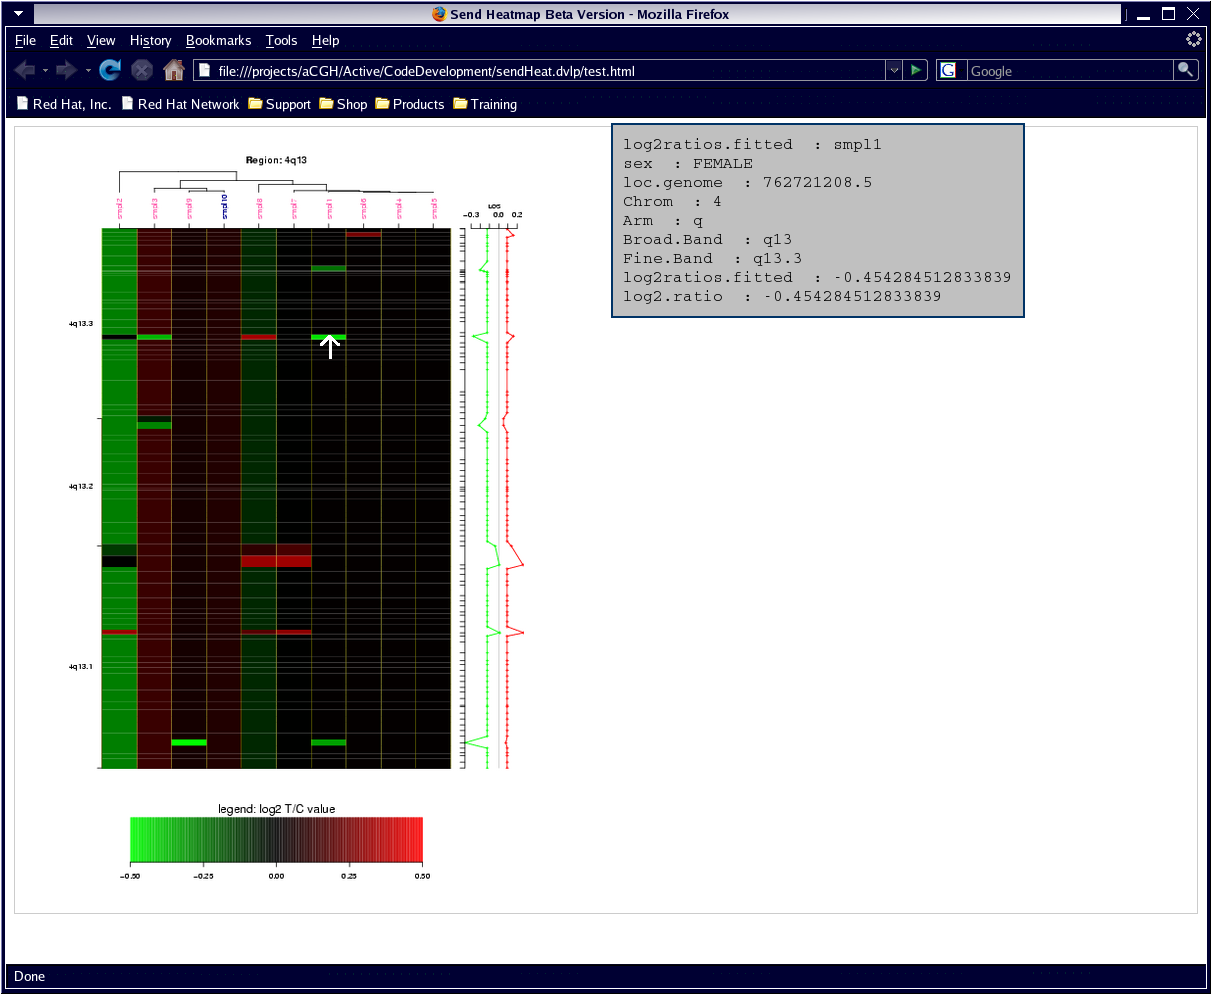
\includegraphics{sendPlot4}
\caption{A snapshot of our example html file opened in Mozilla Firefox. The information is displayed for the region under the white arrow.}
\end{figure}
\end{center}


\end{document}
